\documentclass[a4paper,11pt]{report}

\usepackage[a4paper, total={17cm, 24cm}]{geometry}
% generated by Docutils <http://docutils.sourceforge.net/>
\usepackage{cmap} % fix search and cut-and-paste in Acrobat
\usepackage{ifthen}
\usepackage[T1]{fontenc}
\usepackage[utf8]{inputenc}
\setcounter{secnumdepth}{3}
\usepackage{longtable,ltcaption,array}
\setlength{\extrarowheight}{2pt}
\newlength{\DUtablewidth} % internal use in tables

\usepackage[parfill]{parskip}

%%% Custom LaTeX preamble
% PDF Standard Fonts
\usepackage[scaled=.90]{helvet}
\usepackage{courier}
\usepackage{graphicx}
\graphicspath{{images/}}
\setkeys{Gin}{width=\textwidth}
\usepackage{alltt}
\usepackage{float}
\usepackage{listings}
\lstloadlanguages{csh, python}

%%% MICADO PDR doc packages
\usepackage{dmd-doc}
\usepackage[english]{babel}
\usepackage{multirow}
\usepackage{supertabular}
\usepackage{amsmath}
\usepackage{color}
\definecolor{darkblue}{rgb}{0, 0, 0.5}
\definecolor{listingbg}{gray}{0.95}


%%% User specified packages and stylesheets


%%%%%%%%%%%%%%%%%%%%%%%%%%%%%%%%%%%%%%%%%%%%%%%%%%%%%%%%%%%%%%%%%%%%%%%%%%%%%%%%%
% Docutils-specific commands
%%%%%%%%%%%%%%%%%%%%%%%%%%%%%%%%%%%%%%%%%%%%%%%%%%%%%%%%%%%%%%%%%%%%%%%%%%%%%%%%%


% admonition (specially marked topic)
\providecommand{\DUadmonition}[2][class-arg]{%
  % try \DUadmonition#1{#2}:
  \ifcsname DUadmonition#1\endcsname%
    \csname DUadmonition#1\endcsname{#2}%
  \else
    \begin{center}
      \fbox{\parbox{0.9\linewidth}{#2}}
    \end{center}
  \fi
}

% class handling for environments (block-level elements)
% \begin{DUclass}{spam} tries \DUCLASSspam and
% \end{DUclass}{spam} tries \endDUCLASSspam
\ifx\DUclass\undefined % poor man's "provideenvironment"
 \newenvironment{DUclass}[1]%
  {\def\DocutilsClassFunctionName{DUCLASS#1}% arg cannot be used in end-part of environment.
     \csname \DocutilsClassFunctionName \endcsname}%
  {\csname end\DocutilsClassFunctionName \endcsname}%
\fi

% subtitle (in document title)
\providecommand*{\DUdocumentsubtitle}[1]{{\large #1}}

% title for topics, admonitions, unsupported section levels, and sidebar
\providecommand*{\DUtitle}[2][class-arg]{%
  % call \DUtitle#1{#2} if it exists:
  \ifcsname DUtitle#1\endcsname%
    \csname DUtitle#1\endcsname{#2}%
  \else
    \smallskip\noindent\textbf{#2}\smallskip%
  \fi
}

% hyperlinks:
\ifthenelse{\isundefined{\hypersetup}}{
  \usepackage[colorlinks=true,linkcolor=blue,urlcolor=blue]{hyperref}
  \usepackage{bookmark}
  \urlstyle{same} % normal text font (alternatives: tt, rm, sf)
}{}
\hypersetup{
  pdftitle={ScopeSim instrument packages for MICADO},
}


%%%%%%%%%%%%%%%%%%%%%%%%%%%%%%%%%%%%%%%%%%%%%%%%%%%%%%%%%%%%%%%%%%%%%%%%%%%%%%%%%
% Set title values
%%%%%%%%%%%%%%%%%%%%%%%%%%%%%%%%%%%%%%%%%%%%%%%%%%%%%%%%%%%%%%%%%%%%%%%%%%%%%%%%%

\dmdTitle{ScopeSim instrument packages for MICADO}
\dmdDocId{ELT-TRE-MCD-56306-0059}
\dmdIssue{1.0}
\dmdDate{15. October 2020}
\dmdPreparedBy{K.\ Leschinski}
\dmdPreparedOn{2020-10-15}
\dmdPreparedSig{\resizebox{2.5cm}{!}{
\includegraphics{scribble}}}
\dmdApprovedBy{}
\dmdApprovedOn{}
\dmdApprovedSig{}
\dmdReleasedBy{}
\dmdReleasedOn{}
\dmdReleasedSig{}


%%%%%%%%%%%%%%%%%%%%%%%%%%%%%%%%%%%%%%%%%%%%%%%%%%%%%%%%%%%%%%%%%%%%%%%%%%%%%%%%%
% Body
%%%%%%%%%%%%%%%%%%%%%%%%%%%%%%%%%%%%%%%%%%%%%%%%%%%%%%%%%%%%%%%%%%%%%%%%%%%%%%%%%

\begin{document}

% listings style
\lstset{basicstyle=\ttfamily,
        columns=flexible,
        frame=single,
        backgroundcolor=\color{listingbg},
        captionpos=b,
        showspaces=false}

\dmdmaketitle

%\emptypage{This page was intentionally left blank}

\begin{center}
  \textbf{Change record}

  \tablehead{\hline
    \multicolumn{1}{|c|}{Issue/Rev.} &
    \multicolumn{1}{|c|}{Date} &
    \multicolumn{1}{|c|}{Section/Parag.\ affected} &
    \multicolumn{1}{|c|}{Reason/Initiation/Documents/Remarks} \\
    \hline}
  \tabletail{\hline}

  \begin{supertabular}{|l|l|l|l|}
   0.0.1 & 2020-10-15 & All & (KL) Layout initialised \\
   0.0.2 & 2020-12-04 & All & (KL) Added new data, tables, plots to all sections \\
   \hline
  \end{supertabular}

\end{center}

\begin{center}
  \textbf{Relevant Documents}

  \tablehead{\hline
    \multicolumn{1}{|c|}{Ref. No.} &
    \multicolumn{1}{|c|}{Title} \\
    \hline}
  \tabletail{\hline}

  \begin{supertabular}{|l|l|l|l|}
    &  \\
   \hline
  \end{supertabular}

\end{center}

%\emptypage{This page was unintentionally left blank}

\setcounter{tocdepth}{3}
\tableofcontents
\cleardoublepage


\chapter{Introduction}

\begin{samepage}


\section{Document Scope%
  \label{document-scope}%
}

This document aims to serve as a reference for the contents of the instrument packages relevant to the implementation of the MICADO instrument simulator using the \href{https://scopesim.readthedocs.io/en/latest/}{ScopeSim} package.
The information provided here is a snapshot of the FDR release (Dec. 2020) of the these packages.
It is possible that changes will made to files contained in the packages.
For more up-to-date information, the reader is referred to the \href{https://github.com/astronomyk/irdb}{online GitHub repository}.

This document does not provide an overview of how to use the MICADO packages with \href{https://scopesim.readthedocs.io/en/latest/}{ScopeSim}.
For this the reader should consult the online documentation for \href{https://scopesim.readthedocs.io/en/latest/}{ScopeSim} or either of the two accompanying documents AD\,1 and AD\,2.


\section{Overview of the Instrument Packages relevant to MICADO%
  \label{overview-of-the-instrument-packages-relevant-to-micado}%
}

The MICADO instrument simulator has moved from using the stand alone SimCADO package to using the generic astronomical instrument simulator ScopeSim.
As the ScopeSim code is instrument agnostic, all data related to creating instrument models are contained inside instrument packages, which are hosted on the \href{https://github.com/astronomyk/irdb}{instrument reference database (IRDB)}.


\subsection{Primary MICADO packages%
  \label{primary-micado-packages}%
}

This document is primarily concerned with describing the contents of the two major MICADO instrument descriptions: \texttt{MICADO} and \texttt{MICADO\_Sci}.
These two packages serve two different audiences:

\begin{enumerate}
\item The \texttt{MICADO} package contains all information available pertaining to the optical effects expected for the MICADO optical system.
The primary user of this package will be the data flow system.
The primary use case for this package is the creation of raw data frames for testing the algorithms of the reduction pipelines for the different modes of MICADO.
This package is large and therefore computationally expensive and slow.

\item The \texttt{MICADO\_Sci} package contains a subset of the effects in the \texttt{MICADO} package.
The primary users of this package will be the science team and outside astronomers interested in simulating observations with the future MICADO instrument.
The goal of this package is enable observations to be simulated quickly, so that the user can quickly iterate on observation strategies and/or target choices.
As such this package contains only the effects which cause the major optical aberrations.
It is by nature not complete, but aims to provide a level of detail sufficient for the majority of observation feasibility studies for MICADO
\end{enumerate}


\subsection{Support packages%
  \label{support-packages}%
}

The MICADO packages, as the names suggest, only describe the contents of the MICADO instrument.
Observations with MICADO will however rely on the ELT infrastructure, which can be decomposed into several parts: Location, Telescope, Relay optics.
Each of these additional parts can be considered as closed optical elements in the full observational optical system.
Indeed the relay optics element is a replacable element in the optical path (with MAORY vs stand-alone mode)
Hence each of these optical elements have been given their own instrument package, and are referred to as support packages.

The support packages needed to simulate MICADO observations are also described in this document. Specifically these are:

\begin{itemize}
\item Armazones

\item ELT

\item MAORY

\item Stand-alone relay optics
\end{itemize}

For each observation the Armazones and ELT packages are required. However only one of MAORY or the stand-alone relay optics packages are required.


\subsection{Adding content to the packages%
  \label{adding-content-to-the-packages}%
}

The contents of the packages are currently in the public domain.
The raw data is \href{https://github.com/astronomyk/irdb}{hosted on Github}.

Periodically this data is compiled into an instrument package and uploaded to the ScopeSim server.
It is these packages which are downloaded by ScopeSim when setting up an observation simulation.

New data or Effect objects can be added by submitting a pull request to the \href{https://github.com/astronomyk/irdb}{Github repository}.


\subsection{Contents of packages%
  \label{contents-of-packages}%
}

Each package contains three types of files:

\begin{enumerate}
\item configuration,

\item effect descriptions, and

\item raw data
\end{enumerate}

The configuration files are responsible for controlling which effects and which parameters and values are used when generating the optical model for an observation simulation
The effect files describe which classes and which values should be used when applying an effect to the photon flux of the target object, e.g. which PSF kernel should be applied at which wavelength
The raw dta files provide the raw data needed by the Effect objects, e.g. the bitmaps of the PSF kernels

In the following sections each optical element is described.
Each optical elements contains a description of all the optical Effects associated with it, as well as a list of the configuration keywords and values required by the effect.
If an Effect required data from an external file (e.g. PSF kernels, linearity curves, etc), these data are presented as part of each Effect object - either in the \texttt{Table} or \texttt{Data} sections.

\DUadmonition[note]{
\DUtitle[note]{Note}

The raw data will not always be displayed directly.

A representation of the data will be presented where available.
For further details the reader is directed to the view the data directly on the \href{https://github.com/astronomyk/irdb}{IRDB}
}

\end{samepage}

\chapter{MICADO Pipeline package}

\begin{samepage}


\section{Summary of Effects in Optical Elements:%
  \label{summary-of-effects-in-optical-elements}%
}

\setlength{\DUtablewidth}{\linewidth}
\begin{longtable*}[c]{|p{0.181\DUtablewidth}|p{0.270\DUtablewidth}|p{0.262\DUtablewidth}|p{0.077\DUtablewidth}|p{0.165\DUtablewidth}|}
\hline
\textbf{%
element
} & \textbf{%
name
} & \textbf{%
class
} & \textbf{%
included
} & \textbf{%
z\_orders
} \\
\hline
\endfirsthead
\hline
\textbf{%
element
} & \textbf{%
name
} & \textbf{%
class
} & \textbf{%
included
} & \textbf{%
z\_orders
} \\
\hline
\endhead
\multicolumn{5}{c}{\hfill ... continued on next page} \\
\endfoot
\endlastfoot

armazones
 & 
armazones\_atmo\_default\_ter\_curve
 & 
AtmosphericTERCurve
 & 
True
 & 
{[}111, 511{]}
 \\
\hline

armazones
 & 
armazones\_atmo\_dispersion
 & 
AtmosphericDispersion
 & 
True
 & 
{[}231{]}
 \\
\hline

armazones
 & 
armazones\_atmo\_skycalc\_ter\_curve
 & 
SkycalcTERCurve
 & 
False
 & 
{[}112, 512{]}
 \\
\hline

ELT
 & 
scope\_surface\_list
 & 
SurfaceList
 & 
True
 & 
{[}20, 120, 520{]}
 \\
\hline

ELT
 & 
scope\_vibration
 & 
Vibration
 & 
True
 & 
{[}244, 744{]}
 \\
\hline

ELT
 & 
eso\_combined\_reflection
 & 
TERCurve
 & 
False
 & 
{[}10, 110, 510{]}
 \\
\hline

MICADO
 & 
micado\_static\_surfaces
 & 
SurfaceList
 & 
True
 & 
{[}20, 120, 520{]}
 \\
\hline

MICADO
 & 
micado\_filter
 & 
FilterCurve
 & 
True
 & 
{[}114, 214, 514{]}
 \\
\hline

MICADO
 & 
micado\_ncpas\_psf
 & 
NonCommonPathAberration
 & 
True
 & 
{[}241, 641{]}
 \\
\hline

micado\_detector\_array
 & 
full\_detector\_array
 & 
DetectorList
 & 
False
 & 
{[}90, 290, 390, 490{]}
 \\
\hline

micado\_detector\_array
 & 
detector\_window
 & 
DetectorList
 & 
True
 & 
{[}90, 290, 390, 490{]}
 \\
\hline

micado\_detector\_array
 & 
qe\_curve
 & 
QuantumEfficiencyCurve
 & 
True
 & 
{[}113, 513{]}
 \\
\hline

micado\_detector\_array
 & 
exposure\_action
 & 
SummedExposure
 & 
True
 & 
{[}860{]}
 \\
\hline

micado\_detector\_array
 & 
dark\_current
 & 
DarkCurrent
 & 
True
 & 
{[}830{]}
 \\
\hline

micado\_detector\_array
 & 
detector\_linearity
 & 
LinearityCurve
 & 
True
 & 
{[}840{]}
 \\
\hline

micado\_detector\_array
 & 
shot\_noise
 & 
ShotNoise
 & 
True
 & 
{[}820{]}
 \\
\hline

micado\_detector\_array
 & 
readout\_noise
 & 
PoorMansHxRGReadoutNoise
 & 
True
 & 
{[}811{]}
 \\
\hline

default\_ro
 & 
relay\_psf
 & 
FieldConstantPSF
 & 
True
 & 
{[}262, 662{]}
 \\
\hline

default\_ro
 & 
relay\_surface\_list
 & 
SurfaceList
 & 
True
 & 
{[}20, 120, 520{]}
 \\
\hline

MAORY
 & 
maory\_surface\_list
 & 
SurfaceList
 & 
True
 & 
{[}20, 120, 520{]}
 \\
\hline

MAORY
 & 
maory\_generic\_psf
 & 
FieldConstantPSF
 & 
True
 & 
{[}262, 662{]}
 \\
\hline

MICADO\_IMG\_LR
 & 
micado\_wide\_field\_mirror\_list
 & 
SurfaceList
 & 
True
 & 
{[}20, 120, 520{]}
 \\
\hline

MICADO\_IMG\_LR
 & 
micado\_adc\_3D\_shift
 & 
AtmosphericDispersionCorrection
 & 
True
 & 
{[}632, 232{]}
 \\
\hline

MICADO\_IMG\_HR
 & 
zoom\_mirror\_list
 & 
SurfaceList
 & 
True
 & 
{[}20, 120, 520{]}
 \\
\hline

MICADO\_IMG\_HR
 & 
micado\_adc\_3D\_shift
 & 
AtmosphericDispersionCorrection
 & 
True
 & 
{[}632, 232{]}
 \\
\hline

MICADO\_SPEC
 & 
spec\_mode\_optics
 & 
SurfaceList
 & 
True
 & 
{[}20, 120, 520{]}
 \\
\hline

MICADO\_SPEC
 & 
spectroscopic\_slit\_aperture
 & 
ApertureMask
 & 
True
 & 
{[}80, 280, 380{]}
 \\
\hline

MICADO\_SPEC
 & 
micado\_spectral\_traces
 & 
SpectralTraceList
 & 
True
 & 
{[}70, 270{]}
 \\
\hline

MICADO\_SPEC
 & 
spec\_mode\_optics
 & 
SurfaceList
 & 
True
 & 
{[}20, 120, 520{]}
 \\
\hline

MICADO\_SPEC
 & 
spectroscopic\_slit\_aperture
 & 
ApertureMask
 & 
True
 & 
{[}80, 280, 380{]}
 \\
\hline

MICADO\_SPEC
 & 
micado\_spectral\_traces
 & 
SpectralTraceList
 & 
True
 & 
{[}70, 270{]}
 \\
\hline

MICADO\_SPEC
 & 
spec\_mode\_optics
 & 
SurfaceList
 & 
True
 & 
{[}20, 120, 520{]}
 \\
\hline

MICADO\_SPEC
 & 
spectroscopic\_slit\_aperture
 & 
ApertureMask
 & 
True
 & 
{[}80, 280, 380{]}
 \\
\hline

MICADO\_SPEC
 & 
micado\_spectral\_traces
 & 
SpectralTraceList
 & 
True
 & 
{[}70, 270{]}
 \\
\hline
\end{longtable*}
\label{tbl-effects-summary}



\section{OpticalElement: \textquotedbl{}MICADO\textquotedbl{}%
  \label{opticalelement-micado}%
}

\textbf{Element}: instrument

\textbf{Alias}: INST

\textbf{Description}: Effects from the MICADO common optics


\subsection{Global properties%
  \label{global-properties}%
}

\begin{quote}
\begin{alltt}
\begin{lstlisting}[frame=single]
       temperature : -190
filter_file_format : filters/TC_filter_\{\}.dat
      element_name : MICADO
\end{lstlisting}
\end{alltt}
\end{quote}


\subsection{Effects%
  \label{effects}%
}

Summary of Effects included in this optical element:

\setlength{\DUtablewidth}{\linewidth}
\begin{longtable*}[c]{|p{0.098\DUtablewidth}|p{0.272\DUtablewidth}|p{0.284\DUtablewidth}|p{0.110\DUtablewidth}|p{0.191\DUtablewidth}|}
\hline
\textbf{%
element
} & \textbf{%
name
} & \textbf{%
class
} & \textbf{%
included
} & \textbf{%
z\_orders
} \\
\hline
\endfirsthead
\hline
\textbf{%
element
} & \textbf{%
name
} & \textbf{%
class
} & \textbf{%
included
} & \textbf{%
z\_orders
} \\
\hline
\endhead
\multicolumn{5}{c}{\hfill ... continued on next page} \\
\endfoot
\endlastfoot

MICADO
 & 
micado\_static\_surfaces
 & 
SurfaceList
 & 
True
 & 
{[}20, 120, 520{]}
 \\
\hline

MICADO
 & 
micado\_ncpas\_psf
 & 
NonCommonPathAberration
 & 
True
 & 
{[}241, 641{]}
 \\
\hline

MICADO
 & 
filter\_wheel\_1
 & 
FilterWheel
 & 
True
 & 
{[}124, 224, 524{]}
 \\
\hline

MICADO
 & 
filter\_wheel\_2
 & 
FilterWheel
 & 
True
 & 
{[}124, 224, 524{]}
 \\
\hline

MICADO
 & 
pupil\_wheel
 & 
FilterWheel
 & 
True
 & 
{[}124, 224, 524{]}
 \\
\hline
\end{longtable*}
\label{tbl-micado}


\subsubsection{SurfaceList: \textquotedbl{}micado\_static\_surfaces\textquotedbl{}%
  \label{surfacelist-micado-static-surfaces}%
}

\textbf{Included by default}: \texttt{True}

\textbf{File Description}: surfaces list for wide field optics

\textbf{Class Description}: <no docstring>

\textbf{Changes}:

\begin{itemize}
\item 2019-01-28 (KL) Changed column names and added units to header

\item 2019-07-10 (KL) Shortened the list to only the swappable mirrors

\item 2020-08-25 (KL) Updated angle\_unit to degree from degrees (why has astropy not complained until now?)

\item 2020-10-10 (KL) Added SCAO pick-off dichroic after CM17 conversation
\end{itemize}


\paragraph{Data%
  \label{data}%
}

\begin{figure}[H]
\noindent\makebox[\linewidth][c]{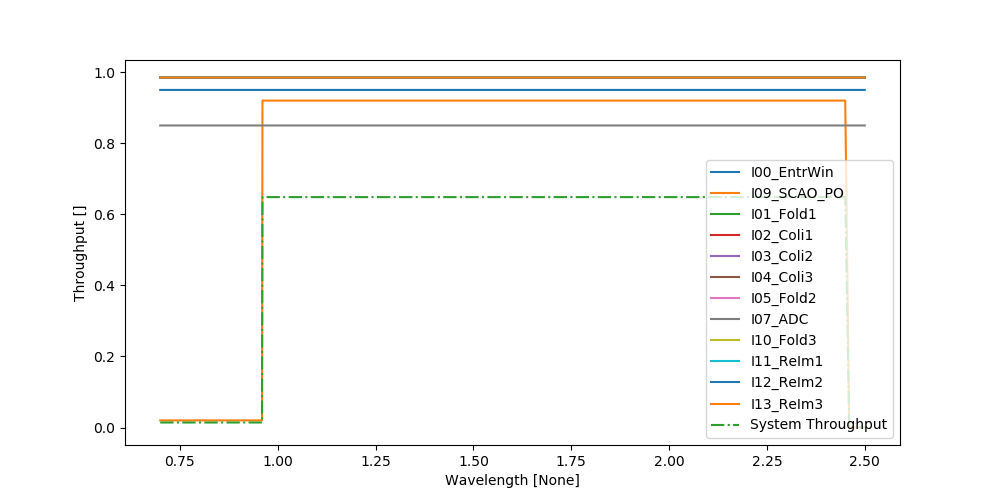
\includegraphics{micado_static_surfaces.png}}\phantomsection\label{fig-micado-static-surfaces}
\end{figure}

\setlength{\DUtablewidth}{\linewidth}
\begin{longtable*}[c]{|p{0.145\DUtablewidth}|p{0.075\DUtablewidth}|p{0.075\DUtablewidth}|p{0.075\DUtablewidth}|p{0.145\DUtablewidth}|p{0.156\DUtablewidth}|p{0.284\DUtablewidth}|}
\hline
\textbf{%
name
} & \textbf{%
outer
} & \textbf{%
inner
} & \textbf{%
angle
} & \textbf{%
temperature
} & \textbf{%
action
} & \textbf{%
filename
} \\
\hline
\endfirsthead
\hline
\textbf{%
name
} & \textbf{%
outer
} & \textbf{%
inner
} & \textbf{%
angle
} & \textbf{%
temperature
} & \textbf{%
action
} & \textbf{%
filename
} \\
\hline
\endhead
\multicolumn{7}{c}{\hfill ... continued on next page} \\
\endfoot
\endlastfoot

I00\_EntrWin
 & 
0.5
 & 
0.0
 & 
0
 & 
0
 & 
transmission
 & 
TER\_entrance\_window.dat
 \\
\hline

I09\_SCAO\_PO
 & 
0.5
 & 
0.0
 & 
45
 & 
-190
 & 
reflection
 & 
TER\_SCAO\_dichroic.dat
 \\
\hline

I01\_Fold1
 & 
0.5
 & 
0.0
 & 
45
 & 
-190
 & 
reflection
 & 
TER\_mirror\_gold.dat
 \\
\hline

I02\_Coli1
 & 
0.4
 & 
0.0
 & 
10
 & 
-190
 & 
reflection
 & 
TER\_mirror\_gold.dat
 \\
\hline

I03\_Coli2
 & 
0.2
 & 
0.0
 & 
10
 & 
-190
 & 
reflection
 & 
TER\_mirror\_gold.dat
 \\
\hline

I04\_Coli3
 & 
0.2
 & 
0.0
 & 
10
 & 
-190
 & 
reflection
 & 
TER\_mirror\_gold.dat
 \\
\hline

I05\_Fold2
 & 
0.2
 & 
0.0
 & 
45
 & 
-190
 & 
reflection
 & 
TER\_mirror\_gold.dat
 \\
\hline

I07\_ADC
 & 
0.2
 & 
0.0
 & 
0
 & 
-190
 & 
transmission
 & 
TER\_full\_adc.dat
 \\
\hline

I10\_Fold3
 & 
0.2
 & 
0.0
 & 
45
 & 
-190
 & 
reflection
 & 
TER\_mirror\_gold.dat
 \\
\hline

I11\_ReIm1
 & 
0.2
 & 
0.0
 & 
10
 & 
-190
 & 
reflection
 & 
TER\_mirror\_gold.dat
 \\
\hline

I12\_ReIm2
 & 
0.2
 & 
0.0
 & 
10
 & 
-190
 & 
reflection
 & 
TER\_mirror\_gold.dat
 \\
\hline

I13\_ReIm3
 & 
0.2
 & 
0.0
 & 
10
 & 
-190
 & 
reflection
 & 
TER\_mirror\_gold.dat
 \\
\hline
\end{longtable*}
\label{tbl-micado-static-surfaces}


\paragraph{Meta-data%
  \label{meta-data}%
}

\begin{quote}
\begin{alltt}
\begin{lstlisting}[frame=single]
            filename : LIST_MICADO_mirrors_static.dat
                name : micado_static_surfaces
         temperature : -190
  filter_file_format : filters/TC_filter_\{\}.dat
        element_name : MICADO
              author : Kieran Leschinski
              source : Ric's SPIE 2018 PPT presentation
        date_created : 2018-11-19
       date_modified : 2019-07-10
              status : Design, pre PDR list of all static MICADO surfaces
                type : mirror:list
          outer_unit : m
          inner_unit : m
          angle_unit : degree
    temperature_unit : deg_C
             z_order : [20, 120, 520]
             include : True
        ignore_wings : False
            wave_min : !SIM.spectral.wave_min
            wave_max : !SIM.spectral.wave_max
           wave_unit : !SIM.spectral.wave_unit
            wave_bin : !SIM.spectral.spectral_resolution
 report_plot_include : True
report_table_include : True
  minimum_throughput : !SIM.spectral.minimum_throughput
             etendue : !TEL.etendue
\end{lstlisting}
\end{alltt}
\end{quote}


\subsubsection{NonCommonPathAberration: \textquotedbl{}micado\_ncpas\_psf\textquotedbl{}%
  \label{noncommonpathaberration-micado-ncpas-psf}%
}

\textbf{Included by default}: \texttt{True}

\textbf{File Description}: Effective NCPA induced PSF kernel

\textbf{Class Description}: Needed: pixel\_scale

\textbf{Changes}:

\begin{itemize}
\item 2018-11-19 (KL) updated meta data to new format
\end{itemize}


\paragraph{Data%
  \label{id1}%
}

\begin{figure}[H]
\noindent\makebox[\linewidth][c]{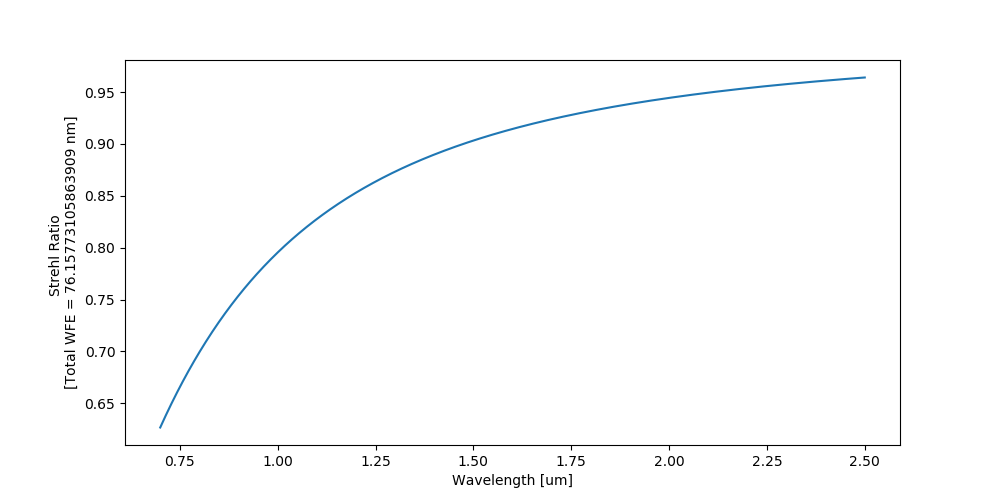
\includegraphics{micado_ncpas_psf.png}}\phantomsection\label{fig-micado-ncpas-psf}
\end{figure}


\paragraph{Meta-data%
  \label{id2}%
}

\begin{quote}
\begin{alltt}
\begin{lstlisting}[frame=single]
            filename : INST_MICADO_wavefront_error_budget.dat
                name : micado_ncpas_psf
         temperature : -190
  filter_file_format : filters/TC_filter_\{\}.dat
        element_name : MICADO
         pixel_scale : 0.004
              author : Kieran Leschinski
             sources : Ric Davies email
        date_created : 2016-11-21
       date_modified : 2018-11-19
                type : instrument:wavefront_errors_list
              status : Idea - based on the WFE budget and emails with Ric
        wfe_rms_unit : nm
             z_order : [241, 641]
             include : True
       flux_accuracy : 0.001
      sub_pixel_flag : False
       convolve_mode : full
            wave_key : WAVE0
    normalise_kernel : True
 report_plot_include : True
report_table_include : False
        kernel_width : None
        strehl_drift : 0.02
            wave_min : !SIM.spectral.wave_min
            wave_max : !SIM.spectral.wave_max
\end{lstlisting}
\end{alltt}
\end{quote}


\subsubsection{FilterWheel: \textquotedbl{}filter\_wheel\_1\textquotedbl{}%
  \label{filterwheel-filter-wheel-1}%
}

\textbf{Included by default}: \texttt{True}

\textbf{File Description}:

\textbf{Class Description}: Examples

\textbf{Changes}:

\begin{itemize}
\item \end{itemize}


\paragraph{Data%
  \label{id3}%
}

\begin{figure}[H]
\noindent\makebox[\linewidth][c]{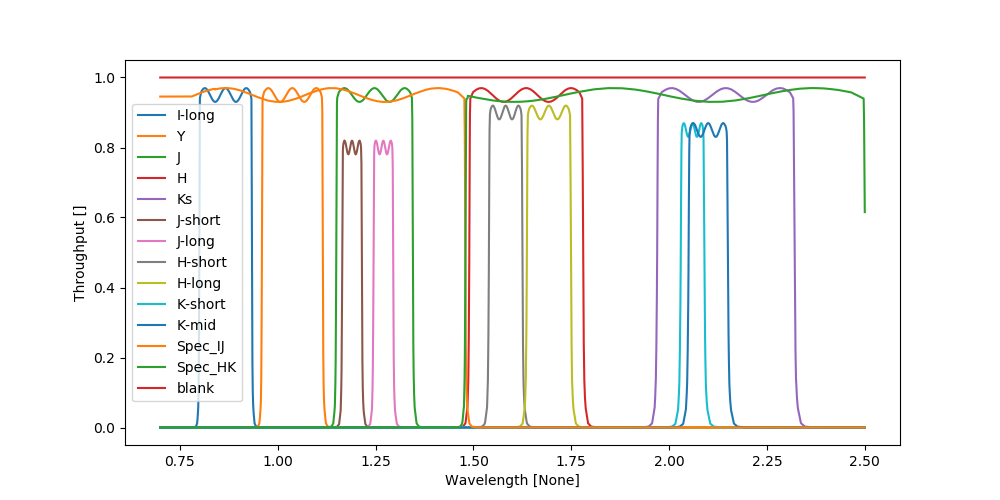
\includegraphics{filter_wheel_1.png}}\phantomsection\label{fig-filter-wheel-1}
\end{figure}

\setlength{\DUtablewidth}{\linewidth}
\begin{longtable*}[c]{|p{0.098\DUtablewidth}|p{0.086\DUtablewidth}|p{0.086\DUtablewidth}|p{0.145\DUtablewidth}|p{0.133\DUtablewidth}|}
\hline
\textbf{%
name
} & \textbf{%
\begin{description}
\item[{centre}] \leavevmode 
um

\end{description}
} & \textbf{%

\begin{description}
\item[{width}] \leavevmode 
um

\end{description}
} & \textbf{%
\begin{description}
\item[{blue cutoff}] \leavevmode 
um

\end{description}
} & \textbf{%
\begin{description}
\item[{red cutoff}] \leavevmode 
um

\end{description}
} \\
\hline
\endfirsthead
\hline
\textbf{%
name
} & \textbf{%
\begin{description}
\item[{centre}] \leavevmode 
um

\end{description}
} & \textbf{%
\begin{description}
\item[{width}] \leavevmode 
um

\end{description}
} & \textbf{%
\begin{description}
\item[{blue cutoff}] \leavevmode 
um

\end{description}
} & \textbf{%
\begin{description}
\item[{red cutoff}] \leavevmode 
um

\end{description}
} \\
\hline
\endhead
\multicolumn{5}{c}{\hfill ... continued on next page} \\
\endfoot
\endlastfoot

I-long
 & 
0.8689
 & 
0.1340
 & 
0.8019
 & 
0.9359
 \\
\hline

Y
 & 
1.0396
 & 
0.1550
 & 
0.9621
 & 
1.1171
 \\
\hline

J
 & 
1.2502
 & 
0.1950
 & 
1.1527
 & 
1.3477
 \\
\hline

H
 & 
1.6395
 & 
0.2900
 & 
1.4945
 & 
1.7845
 \\
\hline

Ks
 & 
2.1500
 & 
0.3500
 & 
1.9750
 & 
2.3250
 \\
\hline

J-short
 & 
1.1902
 & 
0.0490
 & 
1.1657
 & 
1.2147
 \\
\hline

J-long
 & 
1.2702
 & 
0.0490
 & 
1.2457
 & 
1.2947
 \\
\hline

H-short
 & 
1.5830
 & 
0.0850
 & 
1.5405
 & 
1.6255
 \\
\hline

H-long
 & 
1.6937
 & 
0.1120
 & 
1.6377
 & 
1.7497
 \\
\hline

K-short
 & 
2.0602
 & 
0.0600
 & 
2.0302
 & 
2.0902
 \\
\hline

K-mid
 & 
2.1005
 & 
0.1000
 & 
2.0505
 & 
2.1505
 \\
\hline

Spec\_IJ
 & 
1.1663
 & 
0.6990
 & 
0.8168
 & 
1.5158
 \\
\hline

Spec\_HK
 & 
2.0345
 & 
1.0200
 & 
1.5245
 & 
2.5445
 \\
\hline

blank
 & 
2.7545
 & 
2.7000
 & 
1.4045
 & 
4.1045
 \\
\hline
\end{longtable*}
\label{tbl-filter-wheel-1}


\paragraph{Meta-data%
  \label{id4}%
}

\begin{quote}
\begin{alltt}
\begin{lstlisting}[frame=single]
             filename : None
                 name : filter_wheel_1
          temperature : -190
   filter_file_format : filters/TC_filter_\{\}.dat
         element_name : MICADO
         filter_names : ['I-long', 'Y', 'J', 'H', 'Ks', 'J-short', 'J-long', 'H-short', 'H-long', 'K-short', 'K-mid', 'Spec_IJ', 'Spec_HK', 'blank']
      filename_format : !INST.filter_file_format
       current_filter : !OBS.filter_name_fw1
   minimum_throughput : 0.000101
                outer : 0.2
           outer_unit : m
              z_order : [124, 224, 524]
              include : True
                 path :
  report_plot_include : True
 report_table_include : True
report_table_rounding : 4
\end{lstlisting}
\end{alltt}
\end{quote}


\subsubsection{FilterWheel: \textquotedbl{}filter\_wheel\_2\textquotedbl{}%
  \label{filterwheel-filter-wheel-2}%
}

\textbf{Included by default}: \texttt{True}

\textbf{File Description}:

\textbf{Class Description}: Examples

\textbf{Changes}:

\begin{itemize}
\item \end{itemize}


\paragraph{Data%
  \label{id5}%
}

\begin{figure}[H]
\noindent\makebox[\linewidth][c]{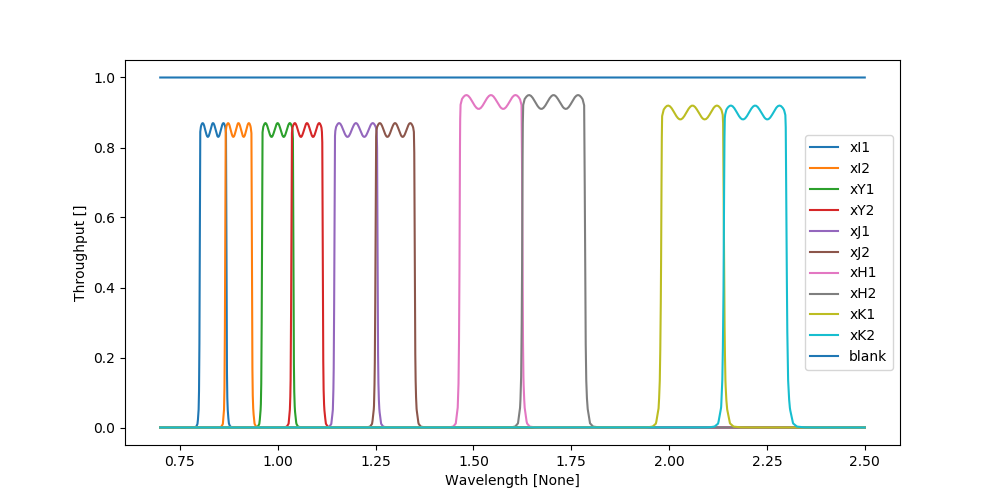
\includegraphics{filter_wheel_2.png}}\phantomsection\label{fig-filter-wheel-2}
\end{figure}

\setlength{\DUtablewidth}{\linewidth}
\begin{longtable*}[c]{|p{0.075\DUtablewidth}|p{0.086\DUtablewidth}|p{0.086\DUtablewidth}|p{0.145\DUtablewidth}|p{0.133\DUtablewidth}|}
\hline
\textbf{%
name
} & \textbf{%
\begin{description}
\item[{centre}] \leavevmode 
um

\end{description}
} & \textbf{%
\begin{description}
\item[{width}] \leavevmode 
um

\end{description}
} & \textbf{%
\begin{description}
\item[{blue cutoff}] \leavevmode 
um

\end{description}
} & \textbf{%
\begin{description}
\item[{red cutoff}] \leavevmode 
um

\end{description}
} \\
\hline
\endfirsthead
\hline
\textbf{%
name
} & \textbf{%
\begin{description}
\item[{centre}] \leavevmode 
um

\end{description}
} & \textbf{%
\begin{description}
\item[{width}] \leavevmode 
um

\end{description}
} & \textbf{%
\begin{description}
\item[{blue cutoff}] \leavevmode 
um

\end{description}
} & \textbf{%
\begin{description}
\item[{red cutoff}] \leavevmode 
um

\end{description}
} \\
\hline
\endhead
\multicolumn{5}{c}{\hfill ... continued on next page} \\
\endfoot
\endlastfoot

xI1
 & 
0.8355
 & 
0.0680
 & 
0.8015
 & 
0.8695
 \\
\hline

xI2
 & 
0.9005
 & 
0.0680
 & 
0.8665
 & 
0.9345
 \\
\hline

xY1
 & 
1.0006
 & 
0.0800
 & 
0.9606
 & 
1.0406
 \\
\hline

xY2
 & 
1.0756
 & 
0.0800
 & 
1.0356
 & 
1.1156
 \\
\hline

xJ1
 & 
1.2009
 & 
0.1100
 & 
1.1459
 & 
1.2559
 \\
\hline

xJ2
 & 
1.3007
 & 
0.1000
 & 
1.2507
 & 
1.3507
 \\
\hline

xH1
 & 
1.5465
 & 
0.1600
 & 
1.4665
 & 
1.6265
 \\
\hline

xH2
 & 
1.7064
 & 
0.1600
 & 
1.6264
 & 
1.7864
 \\
\hline

xK1
 & 
2.0612
 & 
0.1600
 & 
1.9812
 & 
2.1412
 \\
\hline

xK2
 & 
2.2211
 & 
0.1600
 & 
2.1411
 & 
2.3011
 \\
\hline

blank
 & 
2.7545
 & 
2.7000
 & 
1.4045
 & 
4.1045
 \\
\hline
\end{longtable*}
\label{tbl-filter-wheel-2}


\paragraph{Meta-data%
  \label{id6}%
}

\begin{quote}
\begin{alltt}
\begin{lstlisting}[frame=single]
             filename : None
                 name : filter_wheel_2
          temperature : -190
   filter_file_format : filters/TC_filter_\{\}.dat
         element_name : MICADO
         filter_names : ['xI1', 'xI2', 'xY1', 'xY2', 'xJ1', 'xJ2', 'xH1', 'xH2', 'xK1', 'xK2', 'blank']
      filename_format : !INST.filter_file_format
       current_filter : !OBS.filter_name_fw2
   minimum_throughput : 0.000101
                outer : 0.2
           outer_unit : m
              z_order : [124, 224, 524]
              include : True
                 path :
  report_plot_include : True
 report_table_include : True
report_table_rounding : 4
\end{lstlisting}
\end{alltt}
\end{quote}


\subsubsection{FilterWheel: \textquotedbl{}pupil\_wheel\textquotedbl{}%
  \label{filterwheel-pupil-wheel}%
}

\textbf{Included by default}: \texttt{True}

\textbf{File Description}:

\textbf{Class Description}: Examples

\textbf{Changes}:

\begin{itemize}
\item \end{itemize}


\paragraph{Data%
  \label{id7}%
}

\begin{figure}[H]
\noindent\makebox[\linewidth][c]{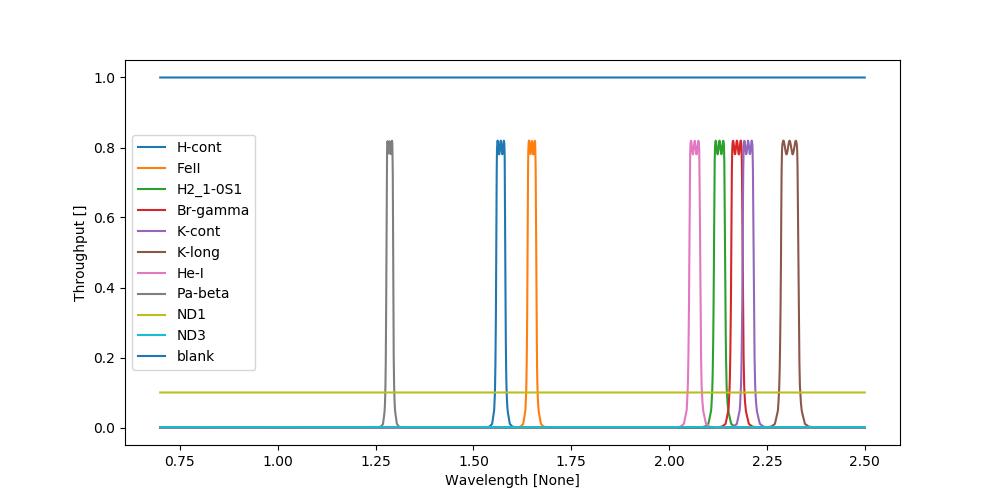
\includegraphics{pupil_wheel.png}}\phantomsection\label{fig-pupil-wheel}
\end{figure}

\setlength{\DUtablewidth}{\linewidth}
\begin{longtable*}[c]{|p{0.110\DUtablewidth}|p{0.086\DUtablewidth}|p{0.086\DUtablewidth}|p{0.145\DUtablewidth}|p{0.133\DUtablewidth}|}
\hline
\textbf{%
name
} & \textbf{%
\begin{description}
\item[{centre}] \leavevmode 
um

\end{description}
} & \textbf{%
\begin{description}
\item[{width}] \leavevmode 
um

\end{description}
} & \textbf{%
\begin{description}
\item[{blue cutoff}] \leavevmode 
um

\end{description}
} & \textbf{%
\begin{description}
\item[{red cutoff}] \leavevmode 
um

\end{description}
} \\
\hline
\endfirsthead
\hline
\textbf{%
name
} & \textbf{%
\begin{description}
\item[{centre}] \leavevmode 
um

\end{description}
} & \textbf{%
\begin{description}
\item[{width}] \leavevmode 
um

\end{description}
} & \textbf{%
\begin{description}
\item[{blue cutoff}] \leavevmode 
um

\end{description}
} & \textbf{%
\begin{description}
\item[{red cutoff}] \leavevmode 
um

\end{description}
} \\
\hline
\endhead
\multicolumn{5}{c}{\hfill ... continued on next page} \\
\endfoot
\endlastfoot

H-cont
 & 
1.5701
 & 
0.0220
 & 
1.5591
 & 
1.5811
 \\
\hline

FeII
 & 
1.6495
 & 
0.0210
 & 
1.6390
 & 
1.6600
 \\
\hline

H2\_1-0S1
 & 
2.1289
 & 
0.0280
 & 
2.1149
 & 
2.1429
 \\
\hline

Br-gamma
 & 
2.1734
 & 
0.0280
 & 
2.1594
 & 
2.1874
 \\
\hline

K-cont
 & 
2.2019
 & 
0.0270
 & 
2.1884
 & 
2.2154
 \\
\hline

K-long
 & 
2.3081
 & 
0.0440
 & 
2.2861
 & 
2.3301
 \\
\hline

He-I
 & 
2.0656
 & 
0.0270
 & 
2.0521
 & 
2.0791
 \\
\hline

Pa-beta
 & 
1.2865
 & 
0.0170
 & 
1.2780
 & 
1.2950
 \\
\hline

ND1
 & 
2.7529
 & 
0.0000
 & 
2.7529
 & 
2.7529
 \\
\hline

ND3
 & 
2.7529
 & 
0.0000
 & 
2.7529
 & 
2.7529
 \\
\hline

blank
 & 
2.7545
 & 
2.7000
 & 
1.4045
 & 
4.1045
 \\
\hline
\end{longtable*}
\label{tbl-pupil-wheel}


\paragraph{Meta-data%
  \label{id8}%
}

\begin{quote}
\begin{alltt}
\begin{lstlisting}[frame=single]
             filename : None
                 name : pupil_wheel
          temperature : -190
   filter_file_format : filters/TC_filter_\{\}.dat
         element_name : MICADO
         filter_names : ['H-cont', 'FeII', 'H2_1-0S1', 'Br-gamma', 'K-cont', 'K-long', 'He-I', 'Pa-beta', 'ND1', 'ND3', 'blank']
      filename_format : !INST.filter_file_format
       current_filter : !OBS.filter_name_pupil
   minimum_throughput : 0.000101
                outer : 0.2
           outer_unit : m
              z_order : [124, 224, 524]
              include : True
                 path :
  report_plot_include : True
 report_table_include : True
report_table_rounding : 4
\end{lstlisting}
\end{alltt}
\end{quote}



\section{OpticalElement: \textquotedbl{}MICADO\_IMG\_LR\textquotedbl{}%
  \label{opticalelement-micado-img-lr}%
}

\textbf{Element}: instrument

\textbf{Alias}: INST

\textbf{Description}: additional effects for the wide-field imaging mode


\subsection{Global properties%
  \label{global-properties}%
}

\begin{quote}
\begin{alltt}
 pixel_scale : 0.004
 plate_scale : 0.26666666666
element_name : MICADO_IMG_LR
\end{alltt}
\end{quote}


\subsection{Effects%
  \label{effects}%
}

Summary of Effects included in this optical element:

\setlength{\DUtablewidth}{\linewidth}
\begin{longtable*}[c]{|p{0.135\DUtablewidth}|p{0.284\DUtablewidth}|p{0.303\DUtablewidth}|p{0.089\DUtablewidth}|p{0.145\DUtablewidth}|}
\hline
\textbf{%
element
} & \textbf{%
name
} & \textbf{%
class
} & \textbf{%
included
} & \textbf{%
z\_orders
} \\
\hline
\endfirsthead
\hline
\textbf{%
element
} & \textbf{%
name
} & \textbf{%
class
} & \textbf{%
included
} & \textbf{%
z\_orders
} \\
\hline
\endhead
\multicolumn{5}{c}{\hfill ... continued on next page} \\
\endfoot
\endlastfoot

MICADO\_IMG\_LR
 & 
micado\_wide\_field\_mirror\_list
 & 
SurfaceList
 & 
True
 & 
{[}20, 120, 520{]}
 \\
\hline

MICADO\_IMG\_LR
 & 
micado\_adc\_3D\_shift
 & 
AtmosphericDispersionCorrection
 & 
True
 & 
{[}632, 232{]}
 \\
\hline
\end{longtable*}
\label{tbl-micado-img-lr}


\subsubsection{SurfaceList: \textquotedbl{}micado\_wide\_field\_mirror\_list\textquotedbl{}%
  \label{surfacelist-micado-wide-field-mirror-list}%
}

\textbf{Included by default}: \texttt{True}

\textbf{File Description}: list of extra mirrors needed for the wide field mode

\textbf{Class Description}: <no docstring>

\textbf{Changes}:

\begin{itemize}
\item \{datetime.date(2019, 1, 28): '(KL) Changed column names and added units to header'\}

\item \{datetime.date(2019, 7, 10): '(KL) Shortened the list to only the swappable mirrors'\}
\end{itemize}


\paragraph{Data%
  \label{data}%
}


\paragraph{Meta-data%
  \label{meta-data}%
}

\begin{quote}
\begin{alltt}
          filename : LIST_MICADO_mirrors_wide.dat
              name : micado_wide_field_mirror_list
       pixel_scale : 0.004
       plate_scale : 0.26666666666
      element_name : MICADO_IMG_LR
            author : Kieran Leschinski
            source : Ric's SPIE 2018 PPT presentation
      date_created : 2018-11-19
     date_modified : 2019-07-10
            status : Design - pre PDR list of MICADO mirrors for wide-field mode
              type : mirror:list
        outer_unit : m
        inner_unit : m
        angle_unit : degree
  temperature_unit : deg_C
           z_order : [20, 120, 520]
           include : True
      ignore_wings : False
          wave_min : !SIM.spectral.wave_min
          wave_max : !SIM.spectral.wave_max
         wave_unit : !SIM.spectral.wave_unit
          wave_bin : !SIM.spectral.spectral_resolution
minimum_throughput : !SIM.spectral.minimum_throughput
           etendue : !TEL.etendue
\end{alltt}
\end{quote}


\subsubsection{AtmosphericDispersionCorrection: \textquotedbl{}micado\_adc\_3D\_shift\textquotedbl{}%
  \label{atmosphericdispersioncorrection-micado-adc-3d-shift}%
}

\textbf{Included by default}: \texttt{True}

\textbf{File Description}: atmospheric disperson corrector

\textbf{Class Description}: <no docstring>

\textbf{Changes}:

\begin{itemize}
\item \end{itemize}


\paragraph{Data%
  \label{id1}%
}


\paragraph{Meta-data%
  \label{id2}%
}

\begin{quote}
\begin{alltt}
    filename : None
        name : micado_adc_3D_shift
 pixel_scale : 0.004
 plate_scale : 0.26666666666
element_name : MICADO_IMG_LR
    altitude : !ATMO.altitude
   longitude : !ATMO.longitude
    latitude : !ATMO.latitude
     airmass : !OBS.airmass
 temperature : !ATMO.temperature
    humidity : !ATMO.humidity
    pressure : !ATMO.pressure
 pupil_angle : !OBS.pupil_angle
  efficiency : 1
    wave_mid : !SIM.spectral.wave_mid
   quick_adc : True
     z_order : [632, 232]
     include : True
\end{alltt}
\end{quote}



\section{OpticalElement: \textquotedbl{}MICADO\_IMG\_HR\textquotedbl{}%
  \label{opticalelement-micado-img-hr}%
}

\textbf{Element}: instrument

\textbf{Alias}: INST

\textbf{Description}: additional effects for the zoom imaging mode


\subsection{Global properties%
  \label{global-properties}%
}

\begin{quote}
\begin{alltt}
 pixel_scale : 0.0015
 plate_scale : 0.1
element_name : MICADO_IMG_HR
\end{alltt}
\end{quote}


\subsection{Effects%
  \label{effects}%
}

Summary of Effects included in this optical element:

\setlength{\DUtablewidth}{\linewidth}
\begin{longtable*}[c]{|p{0.150\DUtablewidth}|p{0.212\DUtablewidth}|p{0.336\DUtablewidth}|p{0.098\DUtablewidth}|p{0.160\DUtablewidth}|}
\hline
\textbf{%
element
} & \textbf{%
name
} & \textbf{%
class
} & \textbf{%
included
} & \textbf{%
z\_orders
} \\
\hline
\endfirsthead
\hline
\textbf{%
element
} & \textbf{%
name
} & \textbf{%
class
} & \textbf{%
included
} & \textbf{%
z\_orders
} \\
\hline
\endhead
\multicolumn{5}{c}{\hfill ... continued on next page} \\
\endfoot
\endlastfoot

MICADO\_IMG\_HR
 & 
zoom\_mirror\_list
 & 
SurfaceList
 & 
True
 & 
{[}20, 120, 520{]}
 \\
\hline

MICADO\_IMG\_HR
 & 
micado\_adc\_3D\_shift
 & 
AtmosphericDispersionCorrection
 & 
True
 & 
{[}632, 232{]}
 \\
\hline
\end{longtable*}
\label{tbl-micado-img-hr}


\subsubsection{SurfaceList: \textquotedbl{}zoom\_mirror\_list\textquotedbl{}%
  \label{surfacelist-zoom-mirror-list}%
}

\textbf{Included by default}: \texttt{True}

\textbf{File Description}: list of extra mirror needed for the zoom imaging mode

\textbf{Class Description}: <no docstring>

\textbf{Changes}:

\begin{itemize}
\item \{datetime.date(2019, 1, 28): '(KL) Changed column names and added units to header'\}

\item \{datetime.date(2019, 7, 10): '(KL) Shortened the list to only the swappable mirrors'\}
\end{itemize}


\paragraph{Data%
  \label{data}%
}


\paragraph{Meta-data%
  \label{meta-data}%
}

\begin{quote}
\begin{alltt}
          filename : LIST_MICADO_mirrors_zoom.dat
              name : zoom_mirror_list
       pixel_scale : 0.0015
       plate_scale : 0.1
      element_name : MICADO_IMG_HR
            author : Kieran Leschinski
            source : Ric's SPIE 2018 PPT presentation
      date_created : 2018-11-19
     date_modified : 2019-07-10
            status : Design - pre PDR list of swappable mirrors for zoom mode
              type : mirror:list
             ETYPE : SURFLIST
              EDIM : 1
        outer_unit : m
        inner_unit : m
        angle_unit : degree
  temperature_unit : deg_C
           z_order : [20, 120, 520]
           include : True
      ignore_wings : False
          wave_min : !SIM.spectral.wave_min
          wave_max : !SIM.spectral.wave_max
         wave_unit : !SIM.spectral.wave_unit
          wave_bin : !SIM.spectral.spectral_resolution
minimum_throughput : !SIM.spectral.minimum_throughput
           etendue : !TEL.etendue
\end{alltt}
\end{quote}


\subsubsection{AtmosphericDispersionCorrection: \textquotedbl{}micado\_adc\_3D\_shift\textquotedbl{}%
  \label{atmosphericdispersioncorrection-micado-adc-3d-shift}%
}

\textbf{Included by default}: \texttt{True}

\textbf{File Description}: atmospheric disperson corrector

\textbf{Class Description}: <no docstring>

\textbf{Changes}:

\begin{itemize}
\item \end{itemize}


\paragraph{Data%
  \label{id1}%
}


\paragraph{Meta-data%
  \label{id2}%
}

\begin{quote}
\begin{alltt}
    filename : None
        name : micado_adc_3D_shift
 pixel_scale : 0.0015
 plate_scale : 0.1
element_name : MICADO_IMG_HR
    altitude : !ATMO.altitude
   longitude : !ATMO.longitude
    latitude : !ATMO.latitude
     airmass : !OBS.airmass
 temperature : !ATMO.temperature
    humidity : !ATMO.humidity
    pressure : !ATMO.pressure
 pupil_angle : !OBS.pupil_angle
    wave_mid : !SIM.spectral.wave_mid
  efficiency : 1
   quick_adc : True
     z_order : [632, 232]
     include : True
\end{alltt}
\end{quote}



\section{OpticalElement: \textquotedbl{}MICADO\_SPEC\textquotedbl{}%
  \label{opticalelement-micado-spec}%
}

\textbf{Element}: instrument

\textbf{Alias}: INST

\textbf{Description}: additional effects for the spectroscopy mode


\subsection{Global properties%
  \label{global-properties}%
}

\begin{quote}
\begin{alltt}
 pixel_scale : 0.004
 plate_scale : 0.2666666667
element_name : MICADO_SPEC
\end{alltt}
\end{quote}


\subsection{Effects%
  \label{effects}%
}

Summary of Effects included in this optical element:

\setlength{\DUtablewidth}{\linewidth}
\begin{longtable*}[c]{|p{0.141\DUtablewidth}|p{0.323\DUtablewidth}|p{0.209\DUtablewidth}|p{0.107\DUtablewidth}|p{0.175\DUtablewidth}|}
\hline
\textbf{%
element
} & \textbf{%
name
} & \textbf{%
class
} & \textbf{%
included
} & \textbf{%
z\_orders
} \\
\hline
\endfirsthead
\hline
\textbf{%
element
} & \textbf{%
name
} & \textbf{%
class
} & \textbf{%
included
} & \textbf{%
z\_orders
} \\
\hline
\endhead
\multicolumn{5}{c}{\hfill ... continued on next page} \\
\endfoot
\endlastfoot

MICADO\_SPEC
 & 
spec\_mode\_optics
 & 
SurfaceList
 & 
True
 & 
{[}20, 120, 520{]}
 \\
\hline

MICADO\_SPEC
 & 
spectroscopic\_slit\_aperture
 & 
ApertureMask
 & 
True
 & 
{[}80, 280, 380{]}
 \\
\hline

MICADO\_SPEC
 & 
micado\_spectral\_traces
 & 
SpectralTraceList
 & 
True
 & 
{[}70, 270{]}
 \\
\hline
\end{longtable*}
\label{tbl-micado-spec}


\subsubsection{SurfaceList: \textquotedbl{}spec\_mode\_optics\textquotedbl{}%
  \label{surfacelist-spec-mode-optics}%
}

\textbf{Included by default}: \texttt{True}

\textbf{File Description}: list of extra mirrors needed for the spectroscopy mode

\textbf{Class Description}: <no docstring>

\textbf{Changes}:

\begin{itemize}
\item \{datetime.date(2019, 1, 28): '(KL) Changed column names and added units to header'\}

\item \{datetime.date(2019, 7, 10): '(KL) Shortened the list to only the swappable gratings'\}
\end{itemize}


\paragraph{Data%
  \label{data}%
}


\paragraph{Meta-data%
  \label{meta-data}%
}

\begin{quote}
\begin{alltt}
          filename : LIST_MICADO_mirrors_spec.dat
              name : spec_mode_optics
       pixel_scale : 0.004
       plate_scale : 0.2666666667
      element_name : MICADO_SPEC
            author : Kieran Leschinski
            source : Ric's SPIE 2018 PPT presentation
      date_created : 2018-11-19
     date_modified : 2019-07-10
            status : Design - pre PDR list of swappable optics for spectroscopy
              type : mirror:list
             ETYPE : SURFLIST
              EDIM : 1
        outer_unit : m
        inner_unit : m
        angle_unit : degree
  temperature_unit : deg_C
           z_order : [20, 120, 520]
           include : True
      ignore_wings : False
          wave_min : !SIM.spectral.wave_min
          wave_max : !SIM.spectral.wave_max
         wave_unit : !SIM.spectral.wave_unit
          wave_bin : !SIM.spectral.spectral_resolution
minimum_throughput : !SIM.spectral.minimum_throughput
           etendue : !TEL.etendue
\end{alltt}
\end{quote}


\subsubsection{ApertureMask: \textquotedbl{}spectroscopic\_slit\_aperture\textquotedbl{}%
  \label{aperturemask-spectroscopic-slit-aperture}%
}

\textbf{Included by default}: \texttt{True}

\textbf{File Description}: Slit mask for the short, narrow slit (3 arcsec x 20 mas)

\textbf{Class Description}: Only provides the on-sky window coords of the Aperture

\textbf{Changes}:

\begin{itemize}
\item \{datetime.date(2019, 7, 10): '(KL) Created the file'\}

\item \{datetime.date(2020, 3, 24): '(KL) Changed geometry to 3000x20mas'\}
\end{itemize}


\paragraph{Data%
  \label{id1}%
}


\paragraph{Meta-data%
  \label{id2}%
}

\begin{quote}
\begin{alltt}
      filename : !OBS.slit_file
          name : spectroscopic_slit_aperture
   pixel_scale : 0.004
   plate_scale : 0.2666666667
  element_name : MICADO_SPEC
        author : Kieran Leschinski
        source : My imagination
  date_created : 2019-07-10
 date_modified : 2019-07-10
        status : Guess - in the train on the way home from CM13
          type : aperture:slit_geometry
        x_unit : arcsec
        y_unit : arcsec
       z_order : [80, 280, 380]
       include : True
       no_mask : True
         angle : 0
         shape : rect
conserve_image : True
            id : 0
\end{alltt}
\end{quote}

<SpectralTrace> \textquotedbl{}list of spectral order trace geometry on the focal plane\textquotedbl{} : {[}1.93, 2.46{]}um : Ext 2 : Aperture 0 : ImagePlane 0
<SpectralTrace> \textquotedbl{}list of spectral order trace geometry on the focal plane\textquotedbl{} : {[}1.45, 1.85{]}um : Ext 3 : Aperture 0 : ImagePlane 0
<SpectralTrace> \textquotedbl{}list of spectral order trace geometry on the focal plane\textquotedbl{} : {[}1.16, 1.48{]}um : Ext 4 : Aperture 0 : ImagePlane 0
<SpectralTrace> \textquotedbl{}list of spectral order trace geometry on the focal plane\textquotedbl{} : {[}1.16, 1.39{]}um : Ext 5 : Aperture 0 : ImagePlane 0
<SpectralTrace> \textquotedbl{}list of spectral order trace geometry on the focal plane\textquotedbl{} : {[}0.97, 1.23{]}um : Ext 6 : Aperture 0 : ImagePlane 0
<SpectralTrace> \textquotedbl{}list of spectral order trace geometry on the focal plane\textquotedbl{} : {[}0.97, 1.23{]}um : Ext 7 : Aperture 0 : ImagePlane 0
<SpectralTrace> \textquotedbl{}list of spectral order trace geometry on the focal plane\textquotedbl{} : {[}0.83, 1.05{]}um : Ext 8 : Aperture 0 : ImagePlane 0
<SpectralTrace> \textquotedbl{}list of spectral order trace geometry on the focal plane\textquotedbl{} : {[}0.83, 1.05{]}um : Ext 9 : Aperture 0 : ImagePlane 0
<SpectralTrace> \textquotedbl{}list of spectral order trace geometry on the focal plane\textquotedbl{} : {[}0.83, 0.92{]}um : Ext 10 : Aperture 0 : ImagePlane 0
<SpectralTrace> \textquotedbl{}list of spectral order trace geometry on the focal plane\textquotedbl{} : {[}0.73, 0.92{]}um : Ext 11 : Aperture 0 : ImagePlane 0
<SpectralTrace> \textquotedbl{}list of spectral order trace geometry on the focal plane\textquotedbl{} : {[}0.73, 0.92{]}um : Ext 12 : Aperture 0 : ImagePlane 0
<SpectralTrace> \textquotedbl{}list of spectral order trace geometry on the focal plane\textquotedbl{} : {[}0.65, 0.82{]}um : Ext 13 : Aperture 0 : ImagePlane 0
<SpectralTrace> \textquotedbl{}list of spectral order trace geometry on the focal plane\textquotedbl{} : {[}0.65, 0.82{]}um : Ext 14 : Aperture 0 : ImagePlane 0
<SpectralTrace> \textquotedbl{}list of spectral order trace geometry on the focal plane\textquotedbl{} : {[}0.6, 0.74{]}um : Ext 15 : Aperture 0 : ImagePlane 0
<SpectralTrace> \textquotedbl{}list of spectral order trace geometry on the focal plane\textquotedbl{} : {[}0.6, 0.73{]}um : Ext 16 : Aperture 0 : ImagePlane 0
<SpectralTrace> \textquotedbl{}list of spectral order trace geometry on the focal plane\textquotedbl{} : {[}0.6, 0.67{]}um : Ext 17 : Aperture 0 : ImagePlane 0
<SpectralTrace> \textquotedbl{}list of spectral order trace geometry on the focal plane\textquotedbl{} : {[}0.6, 0.67{]}um : Ext 18 : Aperture 0 : ImagePlane 0
\textbf{****************************************************************************************************************************************************************************************************************************************************************************************************************************************************************************************************************************************************************************************************************************************************************************************************************************************************************************************************************************************************************************************************************************************************************************************************************************************************************************************************************************************************************************************************************************************************************************************************************************************************************************************************************************************************************************************************************************************************************************************************************************************************************************************************************************************************************************************************************************************************************************************************************************************************************************************************************************************************************************************************************************************************************************************************************************************************************************************************************************************************************}
\textbf{Included by default}: \texttt{True}

\textbf{File Description}: list of spectral order trace geometry on the focal plane

\textbf{Class Description}: List of spectral trace geometries for the detector plane

\textbf{Changes}:

\begin{itemize}
\item \end{itemize}


\paragraph{Data%
  \label{id3}%
}


\paragraph{Meta-data%
  \label{id4}%
}

\begin{quote}
\begin{alltt}
        filename : !OBS.trace_file
            name : micado_spectral_traces
     pixel_scale : 0.004
     plate_scale : 0.2666666667
    element_name : MICADO_SPEC
    wave_colname : lam
       s_colname : xi
col_number_start : 1
   invalid_value : 0
          SIMPLE : True
          BITPIX : 8
           NAXIS : 0
          EXTEND : True
        FILETYPE : Spectral Layout Definition
          AUTHOR : Oliver Czoske
            DATE : 2018-09-16
          SOURCE : Frank Grupp
        ORIGDATE : 2018-06-29
          STATUS : Design PDR
            ECAT : 1
           EDATA : 2
        DESCRIPT : Maps spectral traces from long slit aperture to detector image plane
        DATE_CRE : 2018-06-29
        DATE_MOD : 2019-09-16
         HISTORY : 2019-09-16 : (KL) Added aperture-imagePlane table to EXT 1
         z_order : [70, 270]
         include : True
        wave_min : !SIM.spectral.wave_min
        wave_max : !SIM.spectral.wave_max
       x_colname : x
       y_colname : y
           dwave : 0.002
\end{alltt}
\end{quote}



\section{OpticalElement: \textquotedbl{}micado\_detector\_array\textquotedbl{}%
  \label{opticalelement-micado-detector-array}%
}

\textbf{Element}: detector

\textbf{Alias}: DET

\textbf{Description}: A set of 9 H4RG detectors


\subsection{Global properties%
  \label{global-properties}%
}

\begin{quote}
\begin{alltt}
\begin{lstlisting}[frame=single]
image_plane_id : 0
   temperature : -230
           dit : !OBS.dit
          ndit : !OBS.ndit
  element_name : micado_detector_array
\end{lstlisting}
\end{alltt}
\end{quote}


\subsection{Effects%
  \label{effects}%
}

Summary of Effects included in this optical element:

\setlength{\DUtablewidth}{\linewidth}
\begin{longtable*}[c]{|p{0.218\DUtablewidth}|p{0.199\DUtablewidth}|p{0.247\DUtablewidth}|p{0.092\DUtablewidth}|p{0.199\DUtablewidth}|}
\hline
\textbf{%
element
} & \textbf{%
name
} & \textbf{%
class
} & \textbf{%
included
} & \textbf{%
z\_orders
} \\
\hline
\endfirsthead
\hline
\textbf{%
element
} & \textbf{%
name
} & \textbf{%
class
} & \textbf{%
included
} & \textbf{%
z\_orders
} \\
\hline
\endhead
\multicolumn{5}{c}{\hfill ... continued on next page} \\
\endfoot
\endlastfoot

micado\_detector\_array
 & 
full\_detector\_array
 & 
DetectorList
 & 
False
 & 
{[}90, 290, 390, 490{]}
 \\
\hline

micado\_detector\_array
 & 
detector\_window
 & 
DetectorList
 & 
True
 & 
{[}90, 290, 390, 490{]}
 \\
\hline

micado\_detector\_array
 & 
qe\_curve
 & 
QuantumEfficiencyCurve
 & 
True
 & 
{[}113, 513{]}
 \\
\hline

micado\_detector\_array
 & 
exposure\_action
 & 
SummedExposure
 & 
True
 & 
{[}860{]}
 \\
\hline

micado\_detector\_array
 & 
dark\_current
 & 
DarkCurrent
 & 
True
 & 
{[}830{]}
 \\
\hline

micado\_detector\_array
 & 
detector\_linearity
 & 
LinearityCurve
 & 
True
 & 
{[}840{]}
 \\
\hline

micado\_detector\_array
 & 
shot\_noise
 & 
ShotNoise
 & 
True
 & 
{[}820{]}
 \\
\hline

micado\_detector\_array
 & 
readout\_noise
 & 
PoorMansHxRGReadoutNoise
 & 
True
 & 
{[}811{]}
 \\
\hline
\end{longtable*}
\label{tbl-micado-detector-array}


\subsubsection{DetectorList: \textquotedbl{}full\_detector\_array\textquotedbl{}%
  \label{detectorlist-full-detector-array}%
}

\textbf{Included by default}: \texttt{False}

\textbf{File Description}: MICADO detector array list

\textbf{Class Description}: A description of detector positions and properties

\textbf{Changes}:

\begin{itemize}
\item 2017-08-12 (OC) id changed to conform with spectroscopy report

\item 2018-07-26 (OC) large gap (chips 5 and 6) reduced to 8 mm

\item 2018-11-19 (KL) updated meta data to new format

\item 2019-01-28 (KL) moved units into header
\end{itemize}


\paragraph{Data%
  \label{data}%
}

\begin{figure}[H]
\noindent\makebox[\linewidth][c]{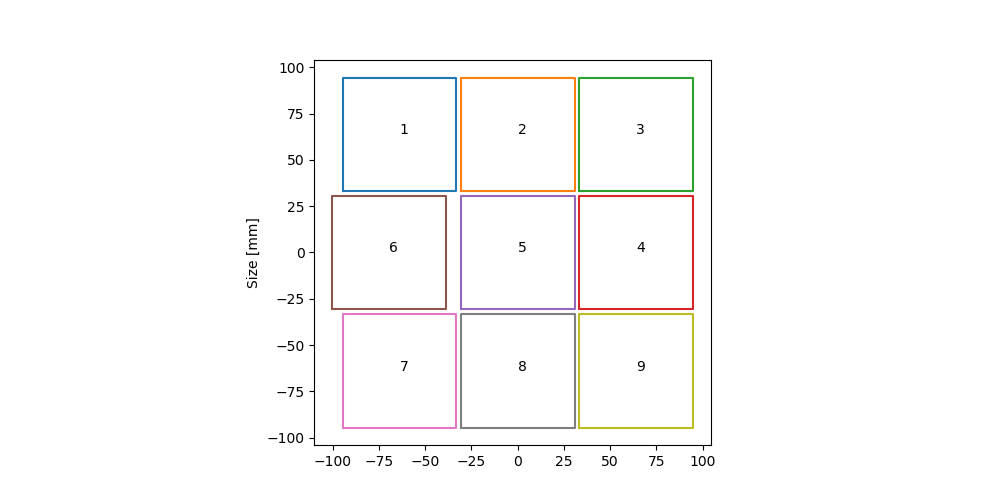
\includegraphics{full_detector_array.png}}\phantomsection\label{fig-full-detector-array}
\end{figure}

\setlength{\DUtablewidth}{\linewidth}
\begin{longtable*}[c]{|p{0.051\DUtablewidth}|p{0.086\DUtablewidth}|p{0.086\DUtablewidth}|p{0.086\DUtablewidth}|p{0.086\DUtablewidth}|p{0.075\DUtablewidth}|p{0.075\DUtablewidth}|p{0.133\DUtablewidth}|p{0.075\DUtablewidth}|p{0.063\DUtablewidth}|}
\hline
\textbf{%
id
} & \textbf{%
x\_cen
} & \textbf{%
y\_cen
} & \textbf{%
x\_size
} & \textbf{%
y\_size
} & \textbf{%
x\_len
} & \textbf{%
y\_len
} & \textbf{%
pixel\_size
} & \textbf{%
angle
} & \textbf{%
gain
} \\
\hline
\endfirsthead
\hline
\textbf{%
id
} & \textbf{%
x\_cen
} & \textbf{%
y\_cen
} & \textbf{%
x\_size
} & \textbf{%
y\_size
} & \textbf{%
x\_len
} & \textbf{%
y\_len
} & \textbf{%
pixel\_size
} & \textbf{%
angle
} & \textbf{%
gain
} \\
\hline
\endhead
\multicolumn{10}{c}{\hfill ... continued on next page} \\
\endfoot
\endlastfoot

1
 & 
-63.84
 & 
63.84
 & 
61.44
 & 
61.44
 & 
4096
 & 
4096
 & 
0.015
 & 
0.0
 & 
1.0
 \\
\hline

2
 & 
0.0
 & 
63.84
 & 
61.44
 & 
61.44
 & 
4096
 & 
4096
 & 
0.015
 & 
0.0
 & 
1.0
 \\
\hline

3
 & 
63.84
 & 
63.84
 & 
61.44
 & 
61.44
 & 
4096
 & 
4096
 & 
0.015
 & 
0.0
 & 
1.0
 \\
\hline

4
 & 
63.84
 & 
0.0
 & 
61.44
 & 
61.44
 & 
4096
 & 
4096
 & 
0.015
 & 
0.0
 & 
1.0
 \\
\hline

5
 & 
0.0
 & 
0.0
 & 
61.44
 & 
61.44
 & 
4096
 & 
4096
 & 
0.015
 & 
0.0
 & 
1.0
 \\
\hline

6
 & 
-69.44
 & 
0.0
 & 
61.44
 & 
61.44
 & 
4096
 & 
4096
 & 
0.015
 & 
0.0
 & 
1.0
 \\
\hline

7
 & 
-63.84
 & 
-63.84
 & 
61.44
 & 
61.44
 & 
4096
 & 
4096
 & 
0.015
 & 
0.0
 & 
1.0
 \\
\hline

8
 & 
0.0
 & 
-63.84
 & 
61.44
 & 
61.44
 & 
4096
 & 
4096
 & 
0.015
 & 
0.0
 & 
1.0
 \\
\hline

9
 & 
63.84
 & 
-63.84
 & 
61.44
 & 
61.44
 & 
4096
 & 
4096
 & 
0.015
 & 
0.0
 & 
1.0
 \\
\hline
\end{longtable*}
\label{tbl-full-detector-array}


\paragraph{Meta-data%
  \label{meta-data}%
}

\begin{quote}
\begin{alltt}
\begin{lstlisting}[frame=single]
            filename : FPA_array_layout.dat
                name : full_detector_array
             include : False
      image_plane_id : 0
         temperature : -230
                 dit : !OBS.dit
                ndit : !OBS.ndit
        element_name : micado_detector_array
    active_detectors : all
              author : Oliver Czoske
             sources : E-MCD-FPA-572089EB.uda, ELT-TRE-MCD-56300-0011
        date_created : 2017-06-28
       date_modified : 2018-07-26
                type : detector:chip_list
          x_cen_unit : mm
          y_cen_unit : mm
            xhw_unit : mm
            yhw_unit : mm
          x_len_unit : pix
          y_len_unit : pix
        pixsize_unit : mm
          angle_unit : deg
           gain_unit : electron/adu
             z_order : [90, 290, 390, 490]
         pixel_scale : !INST.pixel_scale
 report_plot_include : True
report_table_include : True
         x_size_unit : mm
         y_size_unit : mm
\end{lstlisting}
\end{alltt}
\end{quote}


\subsubsection{DetectorList: \textquotedbl{}detector\_window\textquotedbl{}%
  \label{detectorlist-detector-window}%
}

\textbf{Included by default}: \texttt{True}

\textbf{File Description}:

\textbf{Class Description}: A description of detector positions and properties

\textbf{Changes}:

\begin{itemize}
\item \end{itemize}


\paragraph{Data%
  \label{id1}%
}

\begin{figure}[H]
\noindent\makebox[\linewidth][c]{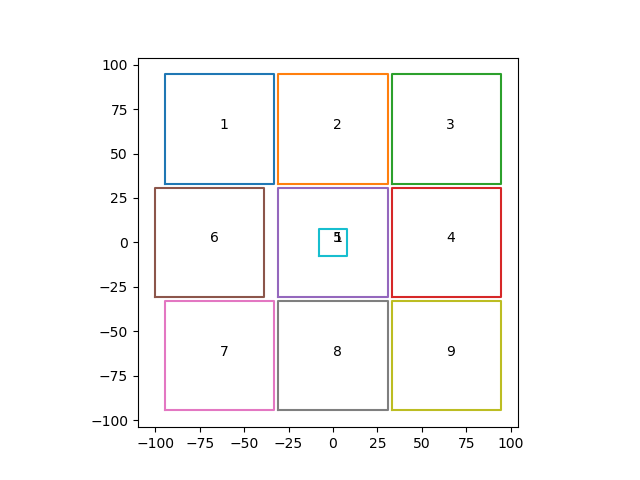
\includegraphics{detector_window.png}}\phantomsection\label{fig-detector-window}
\end{figure}

\setlength{\DUtablewidth}{\linewidth}
\begin{longtable*}[c]{|p{0.051\DUtablewidth}|p{0.133\DUtablewidth}|p{0.075\DUtablewidth}|p{0.063\DUtablewidth}|p{0.075\DUtablewidth}|p{0.075\DUtablewidth}|p{0.086\DUtablewidth}|p{0.086\DUtablewidth}|}
\hline
\textbf{%
id
} & \textbf{%
pixel\_size
} & \textbf{%
angle
} & \textbf{%
gain
} & \textbf{%
x\_cen
} & \textbf{%
y\_cen
} & \textbf{%
x\_size
} & \textbf{%
y\_size
} \\
\hline
\endfirsthead
\hline
\textbf{%
id
} & \textbf{%
pixel\_size
} & \textbf{%
angle
} & \textbf{%
gain
} & \textbf{%
x\_cen
} & \textbf{%
y\_cen
} & \textbf{%
x\_size
} & \textbf{%
y\_size
} \\
\hline
\endhead
\multicolumn{8}{c}{\hfill ... continued on next page} \\
\endfoot
\endlastfoot

1
 & 
0.015
 & 
0.0
 & 
1.0
 & 
0.0
 & 
0.0
 & 
15.36
 & 
15.36
 \\
\hline
\end{longtable*}
\label{tbl-detector-window}


\paragraph{Meta-data%
  \label{id2}%
}

\begin{quote}
\begin{alltt}
\begin{lstlisting}[frame=single]
            filename : None
                name : detector_window
             include : True
      image_plane_id : 0
         temperature : -230
                 dit : !OBS.dit
                ndit : !OBS.ndit
        element_name : micado_detector_array
          x_cen_unit : mm
          y_cen_unit : mm
         x_size_unit : mm
         y_size_unit : mm
     pixel_size_unit : mm
          angle_unit : deg
           gain_unit : electron/adu
             z_order : [90, 290, 390, 490]
          array_dict : \{'id': [1], 'pixel_size': [0.015], 'angle': [0.0], 'gain': [1.0], 'x_cen': [0.0], 'y_cen': [0.0], 'x_size': [15.36], 'y_size': [15.36]\}
         pixel_scale : !INST.pixel_scale
    active_detectors : all
 report_plot_include : True
report_table_include : True
\end{lstlisting}
\end{alltt}
\end{quote}


\subsubsection{QuantumEfficiencyCurve: \textquotedbl{}qe\_curve\textquotedbl{}%
  \label{quantumefficiencycurve-qe-curve}%
}

\textbf{Included by default}: \texttt{True}

\textbf{File Description}: Quantum efficiency curves for each detector

\textbf{Class Description}: <no docstring>

\textbf{Changes}:

\begin{itemize}
\item 2018-11-19 (KL) updated meta data to new format

\item 2019-08-09 (KL) Added action keyword to meta data
\end{itemize}


\paragraph{Data%
  \label{id3}%
}

\begin{figure}[H]
\noindent\makebox[\linewidth][c]{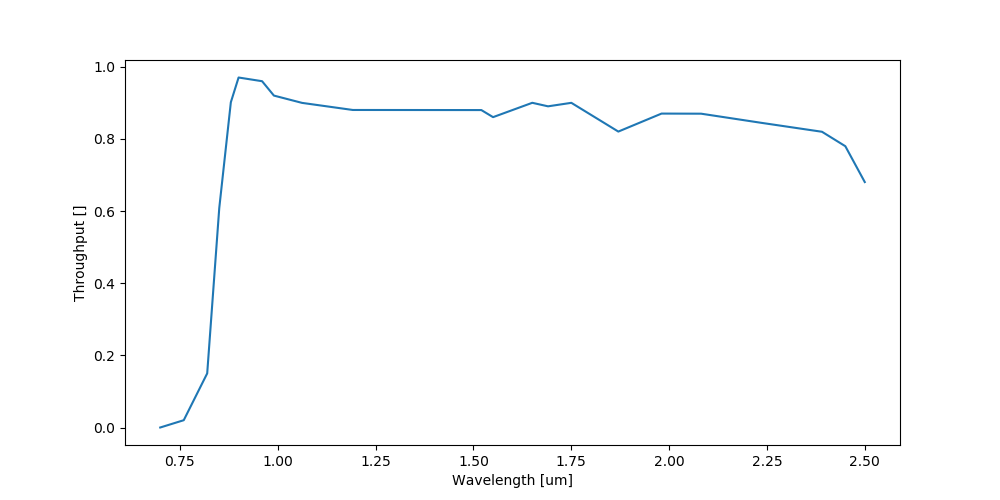
\includegraphics{qe_curve.png}}\phantomsection\label{fig-qe-curve}
\end{figure}


\paragraph{Meta-data%
  \label{id4}%
}

\begin{quote}
\begin{alltt}
\begin{lstlisting}[frame=single]
            filename : QE_detector_H2RG.dat
                name : qe_curve
      image_plane_id : 0
         temperature : -230
                 dit : 60
                ndit : 1
        element_name : micado_detector_array
              author : Kieran Leschinski
             sources : Finger+ 2008 SPIE
        date_created : 2016-01-01
       date_modified : 2019-08-09
                type : detector:quantum_efficiency
              status : Design, guestimated by reading off the graph in Finger+ 2008
     wavelength_unit : um
              action : transmission
             z_order : [113, 513]
             include : True
        ignore_wings : False
            wave_min : 0.7
            wave_max : 2.5
           wave_unit : um
            wave_bin : 0.0001
 report_plot_include : True
report_table_include : False
            position : -1
\end{lstlisting}
\end{alltt}
\end{quote}


\subsubsection{SummedExposure: \textquotedbl{}exposure\_action\textquotedbl{}%
  \label{summedexposure-exposure-action}%
}

\textbf{Included by default}: \texttt{True}

\textbf{File Description}: Summing up sky signal for all DITs and NDITs

\textbf{Class Description}: Simulates a summed stack of \texttt{ndit} exposures

\textbf{Changes}:

\begin{itemize}
\item \end{itemize}


\paragraph{Data%
  \label{id5}%
}


\paragraph{Meta-data%
  \label{id6}%
}

\begin{quote}
\begin{alltt}
\begin{lstlisting}[frame=single]
      filename : None
          name : exposure_action
image_plane_id : 0
   temperature : -230
           dit : !OBS.dit
          ndit : !OBS.ndit
  element_name : micado_detector_array
       z_order : [860]
       include : True
\end{lstlisting}
\end{alltt}
\end{quote}


\subsubsection{DarkCurrent: \textquotedbl{}dark\_current\textquotedbl{}%
  \label{darkcurrent-dark-current}%
}

\textbf{Included by default}: \texttt{True}

\textbf{File Description}: MICADO dark current

\textbf{Class Description}: required: dit, ndit, value

\textbf{Changes}:

\begin{itemize}
\item \end{itemize}


\paragraph{Data%
  \label{id7}%
}


\paragraph{Meta-data%
  \label{id8}%
}

\begin{quote}
\begin{alltt}
\begin{lstlisting}[frame=single]
      filename : None
          name : dark_current
image_plane_id : 0
   temperature : -230
           dit : !OBS.dit
          ndit : !OBS.ndit
  element_name : micado_detector_array
         value : 0.1
       z_order : [830]
       include : True
\end{lstlisting}
\end{alltt}
\end{quote}


\subsubsection{LinearityCurve: \textquotedbl{}detector\_linearity\textquotedbl{}%
  \label{linearitycurve-detector-linearity}%
}

\textbf{Included by default}: \texttt{True}

\textbf{File Description}: Linearity characteristics of H4RG chips

\textbf{Class Description}: <no docstring>

\textbf{Changes}:

\begin{itemize}
\item 2018-11-19 (KL) updated meta data to new format

\item 2019-08-14 (KL) replaced long 1000000000 with 1e99
\end{itemize}


\paragraph{Data%
  \label{id9}%
}

\begin{figure}[H]
\noindent\makebox[\linewidth][c]{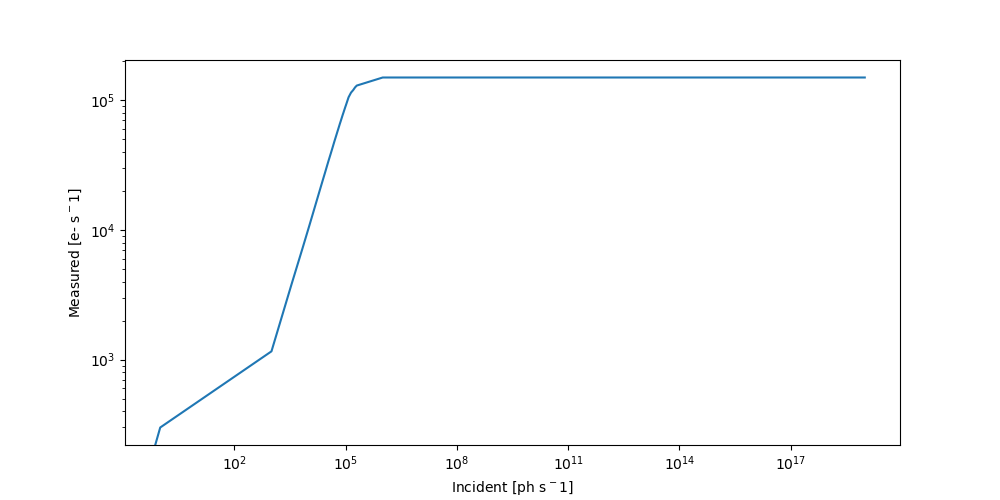
\includegraphics{detector_linearity.png}}\phantomsection\label{fig-detector-linearity}
\end{figure}


\paragraph{Meta-data%
  \label{id10}%
}

\begin{quote}
\begin{alltt}
\begin{lstlisting}[frame=single]
            filename : FPA_linearity.dat
                name : detector_linearity
      image_plane_id : 0
         temperature : -230
                 dit : !OBS.dit
                ndit : !OBS.ndit
        element_name : micado_detector_array
              author : Kieran Leschinski
             sources : Ingraham+ 2014 - Gemini Calibrations II for H2RG
        date_created : 2016-01-01
       date_modified : 2018-11-19
                type : detector:linearity
              status : Design, approximated from the H2RG
       incident_unit : ph
       measured_unit : ph
             z_order : [840]
             include : True
 report_plot_include : True
report_table_include : False
\end{lstlisting}
\end{alltt}
\end{quote}


\subsubsection{ShotNoise: \textquotedbl{}shot\_noise\textquotedbl{}%
  \label{shotnoise-shot-noise}%
}

\textbf{Included by default}: \texttt{True}

\textbf{File Description}: apply poisson shot noise to images

\textbf{Class Description}: <no docstring>

\textbf{Changes}:

\begin{itemize}
\item \end{itemize}


\paragraph{Data%
  \label{id11}%
}


\paragraph{Meta-data%
  \label{id12}%
}

\begin{quote}
\begin{alltt}
\begin{lstlisting}[frame=single]
      filename : None
          name : shot_noise
image_plane_id : 0
   temperature : -230
           dit : !OBS.dit
          ndit : !OBS.ndit
  element_name : micado_detector_array
       z_order : [820]
       include : True
   random_seed : !SIM.random.seed
\end{lstlisting}
\end{alltt}
\end{quote}


\subsubsection{PoorMansHxRGReadoutNoise: \textquotedbl{}readout\_noise\textquotedbl{}%
  \label{poormanshxrgreadoutnoise-readout-noise}%
}

\textbf{Included by default}: \texttt{True}

\textbf{File Description}: Readout noise frames

\textbf{Class Description}: <no docstring>

\textbf{Changes}:

\begin{itemize}
\item \end{itemize}


\paragraph{Data%
  \label{id13}%
}


\paragraph{Meta-data%
  \label{id14}%
}

\begin{quote}
\begin{alltt}
\begin{lstlisting}[frame=single]
            filename : None
                name : readout_noise
      image_plane_id : 0
         temperature : -230
                 dit : !OBS.dit
                ndit : !OBS.ndit
        element_name : micado_detector_array
           noise_std : 12
          n_channels : 64
             z_order : [811]
             include : True
   pedestal_fraction : 0.3
       read_fraction : 0.4
       line_fraction : 0.25
    channel_fraction : 0.05
         random_seed : !SIM.random.seed
 report_plot_include : False
report_table_include : False
\end{lstlisting}
\end{alltt}
\end{quote}



\section{OpticalElement: \textquotedbl{}MICADO\_simulation\_paramters\textquotedbl{}%
  \label{opticalelement-micado-simulation-paramters}%
}

\textbf{Element}: simulation

\textbf{Alias}: SIM

\textbf{Description}: RC simulation paramters which need to change for a MICADO run


\subsection{Global properties%
  \label{global-properties}%
}

\begin{quote}
\begin{alltt}
\begin{lstlisting}[frame=single]
      random : \{'seed': 9001\}
    spectral : \{'wave_min': 0.7, 'wave_mid': 1.6, 'wave_max': 2.5\}
   computing : \{'preload_field_of_view': True\}
     reports : \{'preamble_file': '../docs/preamble.rst'\}
element_name : MICADO_simulation_paramters
\end{lstlisting}
\end{alltt}
\end{quote}

\end{samepage}

\chapter{MICADO Science package}

\begin{samepage}


\section{Summary of Effects in Optical Elements:%
  \label{summary-of-effects-in-optical-elements}%
}

\setlength{\DUtablewidth}{\linewidth}
\begin{longtable*}[c]{|p{0.199\DUtablewidth}|p{0.218\DUtablewidth}|p{0.247\DUtablewidth}|p{0.092\DUtablewidth}|p{0.199\DUtablewidth}|}
\hline
\textbf{%
element
} & \textbf{%
name
} & \textbf{%
class
} & \textbf{%
included
} & \textbf{%
z\_orders
} \\
\hline
\endfirsthead
\hline
\textbf{%
element
} & \textbf{%
name
} & \textbf{%
class
} & \textbf{%
included
} & \textbf{%
z\_orders
} \\
\hline
\endhead
\multicolumn{5}{c}{\hfill ... continued on next page} \\
\endfoot
\endlastfoot

MICADO
 & 
micado\_filter
 & 
FilterCurve
 & 
True
 & 
{[}114, 214, 514{]}
 \\
\hline

MICADO
 & 
micado\_common\_optics
 & 
TERCurve
 & 
True
 & 
{[}10, 110, 510{]}
 \\
\hline

micado\_sci\_detector
 & 
detector\_window
 & 
DetectorWindow
 & 
True
 & 
{[}90, 290, 390, 490{]}
 \\
\hline

micado\_sci\_detector
 & 
qe\_curve
 & 
QuantumEfficiencyCurve
 & 
True
 & 
{[}113, 513{]}
 \\
\hline

micado\_sci\_detector
 & 
exposure\_action
 & 
SummedExposure
 & 
True
 & 
{[}860{]}
 \\
\hline

micado\_sci\_detector
 & 
dark\_current
 & 
DarkCurrent
 & 
True
 & 
{[}830{]}
 \\
\hline

micado\_sci\_detector
 & 
shot\_noise
 & 
ShotNoise
 & 
True
 & 
{[}820{]}
 \\
\hline

micado\_sci\_detector
 & 
readout\_noise
 & 
PoorMansHxRGReadoutNoise
 & 
True
 & 
{[}811{]}
 \\
\hline

MICADO\_SCAO
 & 
scao\_relay\_optics\_ter
 & 
TERCurve
 & 
True
 & 
{[}10, 110, 510{]}
 \\
\hline

MICADO\_SCAO
 & 
scao\_const\_psf
 & 
AnisocadoConstPSF
 & 
True
 & 
{[}42{]}
 \\
\hline

MICADO\_MCAO
 & 
maory\_mms\_ter
 & 
TERCurve
 & 
True
 & 
{[}10, 110, 510{]}
 \\
\hline

MICADO\_MCAO
 & 
maory\_const\_psf
 & 
AnisocadoConstPSF
 & 
True
 & 
{[}42{]}
 \\
\hline
\end{longtable*}
\label{tbl-effects-summary}



\section{OpticalElement: \textquotedbl{}MICADO\_Sci\textquotedbl{}%
  \label{opticalelement-micado-sci}%
}

\textbf{Element}: instrument

\textbf{Alias}: INST

\textbf{Description}: base configuration for MICADO


\subsection{Global properties%
  \label{global-properties}%
}

\begin{quote}
\begin{alltt}
\begin{lstlisting}[frame=single]
       temperature : -190
filter_file_format : filters/TC_filter_\{\}.dat
      element_name : MICADO_Sci
\end{lstlisting}
\end{alltt}
\end{quote}


\subsection{Effects%
  \label{effects}%
}

Summary of Effects included in this optical element:

\setlength{\DUtablewidth}{\linewidth}
\begin{longtable*}[c]{|p{0.133\DUtablewidth}|p{0.249\DUtablewidth}|p{0.145\DUtablewidth}|p{0.110\DUtablewidth}|p{0.156\DUtablewidth}|}
\hline
\textbf{%
element
} & \textbf{%
name
} & \textbf{%
class
} & \textbf{%
included
} & \textbf{%
z\_orders {[}3{]}
} \\
\hline
\endfirsthead
\hline
\textbf{%
element
} & \textbf{%
name
} & \textbf{%
class
} & \textbf{%
included
} & \textbf{%
z\_orders {[}3{]}
} \\
\hline
\endhead
\multicolumn{5}{c}{\hfill ... continued on next page} \\
\endfoot
\endlastfoot

MICADO\_Sci
 & 
micado\_common\_optics
 & 
TERCurve
 & 
True
 & 
10 .. 510
 \\
\hline

MICADO\_Sci
 & 
filter\_wheel
 & 
FilterWheel
 & 
True
 & 
124 .. 524
 \\
\hline
\end{longtable*}
\label{tbl-micado-sci}


\subsubsection{TERCurve: \textquotedbl{}micado\_common\_optics\textquotedbl{}%
  \label{tercurve-micado-common-optics}%
}

\textbf{Included by default}: \texttt{True}

\textbf{File Description}: combined transmission for MICADO common optics

\textbf{Class Description}: Transmission, Emissivity, Reflection Curve

\textbf{Changes}:

\begin{itemize}
\item \end{itemize}


\paragraph{Data%
  \label{data}%
}

\begin{figure}[H]
\noindent\makebox[\linewidth][c]{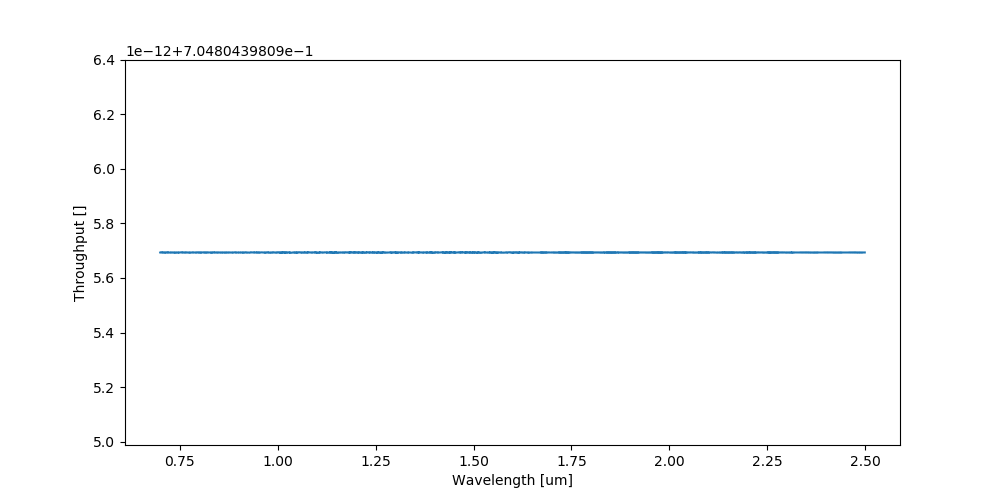
\includegraphics{micado_common_optics.png}}\phantomsection\label{fig-micado-common-optics}
\end{figure}


\paragraph{Meta-data%
  \label{meta-data}%
}

\begin{quote}
\begin{alltt}
\begin{lstlisting}[frame=single]
            filename : TER_MICADO_IMG_common.dat
                name : micado_common_optics
         temperature : -190
  filter_file_format : filters/TC_filter_\{\}.dat
        element_name : MICADO_Sci
              author : Auto-compiled from source
              source : LIST_MICADO_mirrors_static.dat
        date_created : 2020-08-25
       date_modified : 2020-08-25
                area : 0.19634954084936207
           area_unit : m2
     wavelength_unit : um
       emission_unit : photlam
             z_order : [10, 110, 510]
             include : True
        ignore_wings : False
            wave_min : 0.7
            wave_max : 2.5
           wave_unit : um
            wave_bin : 0.001
 report_plot_include : True
report_table_include : False
\end{lstlisting}
\end{alltt}
\end{quote}


\subsubsection{FilterWheel: \textquotedbl{}filter\_wheel\textquotedbl{}%
  \label{filterwheel-filter-wheel}%
}

\textbf{Included by default}: \texttt{True}

\textbf{File Description}:

\textbf{Class Description}: Examples

\textbf{Changes}:

\begin{itemize}
\item \end{itemize}


\paragraph{Data%
  \label{id1}%
}

\begin{figure}[H]
\noindent\makebox[\linewidth][c]{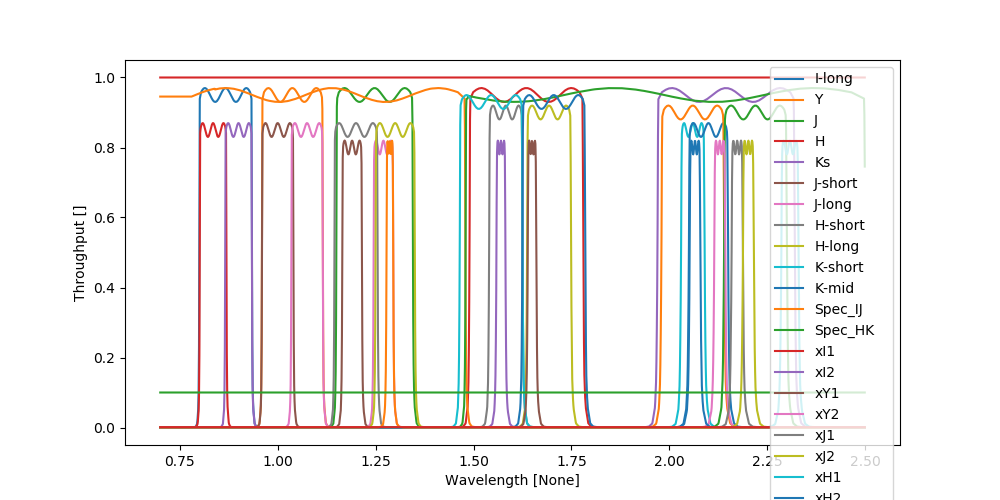
\includegraphics{filter_wheel.png}}\phantomsection\label{fig-filter-wheel}
\end{figure}

\setlength{\DUtablewidth}{\linewidth}
\begin{longtable*}[c]{|p{0.110\DUtablewidth}|p{0.086\DUtablewidth}|p{0.086\DUtablewidth}|p{0.145\DUtablewidth}|p{0.133\DUtablewidth}|}
\hline
\textbf{%
name
} & \textbf{%
\begin{description}
\item[{centre}] \leavevmode 
um

\end{description}
} & \textbf{%
\begin{description}
\item[{width}] \leavevmode 
um

\end{description}
} & \textbf{%
\begin{description}
\item[{blue cutoff}] \leavevmode 
um

\end{description}
} & \textbf{%
\begin{description}
\item[{red cutoff}] \leavevmode 
um

\end{description}
} \\
\hline
\endfirsthead
\hline
\textbf{%
name
} & \textbf{%
\begin{description}
\item[{centre}] \leavevmode 
um

\end{description}
} & \textbf{%
\begin{description}
\item[{width}] \leavevmode 
um

\end{description}
} & \textbf{%
\begin{description}
\item[{blue cutoff}] \leavevmode 
um

\end{description}
} & \textbf{%
\begin{description}
\item[{red cutoff}] \leavevmode 
um

\end{description}
} \\
\hline
\endhead
\multicolumn{5}{c}{\hfill ... continued on next page} \\
\endfoot
\endlastfoot

I-long
 & 
0.8689
 & 
0.1340
 & 
0.8019
 & 
0.9359
 \\
\hline

Y
 & 
1.0396
 & 
0.1550
 & 
0.9621
 & 
1.1171
 \\
\hline

J
 & 
1.2502
 & 
0.1950
 & 
1.1527
 & 
1.3477
 \\
\hline

H
 & 
1.6395
 & 
0.2900
 & 
1.4945
 & 
1.7845
 \\
\hline

Ks
 & 
2.1500
 & 
0.3500
 & 
1.9750
 & 
2.3250
 \\
\hline

J-short
 & 
1.1902
 & 
0.0490
 & 
1.1657
 & 
1.2147
 \\
\hline

J-long
 & 
1.2702
 & 
0.0490
 & 
1.2457
 & 
1.2947
 \\
\hline

H-short
 & 
1.5830
 & 
0.0850
 & 
1.5405
 & 
1.6255
 \\
\hline

H-long
 & 
1.6937
 & 
0.1120
 & 
1.6377
 & 
1.7497
 \\
\hline

K-short
 & 
2.0602
 & 
0.0600
 & 
2.0302
 & 
2.0902
 \\
\hline

K-mid
 & 
2.1005
 & 
0.1000
 & 
2.0505
 & 
2.1505
 \\
\hline

Spec\_IJ
 & 
1.1663
 & 
0.6990
 & 
0.8168
 & 
1.5158
 \\
\hline

Spec\_HK
 & 
2.0345
 & 
1.0200
 & 
1.5245
 & 
2.5445
 \\
\hline

xI1
 & 
0.8355
 & 
0.0680
 & 
0.8015
 & 
0.8695
 \\
\hline

xI2
 & 
0.9005
 & 
0.0680
 & 
0.8665
 & 
0.9345
 \\
\hline

xY1
 & 
1.0006
 & 
0.0800
 & 
0.9606
 & 
1.0406
 \\
\hline

xY2
 & 
1.0756
 & 
0.0800
 & 
1.0356
 & 
1.1156
 \\
\hline

xJ1
 & 
1.2009
 & 
0.1100
 & 
1.1459
 & 
1.2559
 \\
\hline

xJ2
 & 
1.3007
 & 
0.1000
 & 
1.2507
 & 
1.3507
 \\
\hline

xH1
 & 
1.5465
 & 
0.1600
 & 
1.4665
 & 
1.6265
 \\
\hline

xH2
 & 
1.7064
 & 
0.1600
 & 
1.6264
 & 
1.7864
 \\
\hline

xK1
 & 
2.0612
 & 
0.1600
 & 
1.9812
 & 
2.1412
 \\
\hline

xK2
 & 
2.2211
 & 
0.1600
 & 
2.1411
 & 
2.3011
 \\
\hline

blank
 & 
2.7545
 & 
2.7000
 & 
1.4045
 & 
4.1045
 \\
\hline

H-cont
 & 
1.5701
 & 
0.0220
 & 
1.5591
 & 
1.5811
 \\
\hline

FeII
 & 
1.6495
 & 
0.0210
 & 
1.6390
 & 
1.6600
 \\
\hline

H2\_1-0S1
 & 
2.1289
 & 
0.0280
 & 
2.1149
 & 
2.1429
 \\
\hline

Br-gamma
 & 
2.1734
 & 
0.0280
 & 
2.1594
 & 
2.1874
 \\
\hline

K-cont
 & 
2.2019
 & 
0.0270
 & 
2.1884
 & 
2.2154
 \\
\hline

K-long
 & 
2.3081
 & 
0.0440
 & 
2.2861
 & 
2.3301
 \\
\hline

He-I
 & 
2.0656
 & 
0.0270
 & 
2.0521
 & 
2.0791
 \\
\hline

Pa-beta
 & 
1.2865
 & 
0.0170
 & 
1.2780
 & 
1.2950
 \\
\hline

ND1
 & 
2.7529
 & 
0.0000
 & 
2.7529
 & 
2.7529
 \\
\hline

ND3
 & 
2.7529
 & 
0.0000
 & 
2.7529
 & 
2.7529
 \\
\hline
\end{longtable*}
\label{tbl-filter-wheel}


\paragraph{Meta-data%
  \label{id2}%
}

\begin{quote}
\begin{alltt}
\begin{lstlisting}[frame=single]
             filename : None
                 name : filter_wheel
          temperature : -190
   filter_file_format : filters/TC_filter_\{\}.dat
         element_name : MICADO_Sci
         filter_names : ['I-long', 'Y', 'J', 'H', 'Ks', 'J-short', 'J-long', 'H-short', 'H-long', 'K-short', 'K-mid', 'Spec_IJ', 'Spec_HK', 'xI1', 'xI2', 'xY1', 'xY2', 'xJ1', 'xJ2', 'xH1', 'xH2', 'xK1', 'xK2', 'blank', 'H-cont', 'FeII', 'H2_1-0S1', 'Br-gamma', 'K-cont', 'K-long', 'He-I', 'Pa-beta', 'ND1', 'ND3']
      filename_format : !INST.filter_file_format
       current_filter : !INST.filter_name
   minimum_throughput : 0.000101
                outer : 0.2
           outer_unit : m
              z_order : [124, 224, 524]
              include : True
                 path :
  report_plot_include : True
 report_table_include : True
report_table_rounding : 4
\end{lstlisting}
\end{alltt}
\end{quote}



\section{OpticalElement: \textquotedbl{}SCAO\textquotedbl{}%
  \label{opticalelement-scao}%
}

\textbf{Element}: instrument

\textbf{Alias}: INST

\textbf{Description}: SCAO optical system


\subsection{Global properties%
  \label{global-properties}%
}

\begin{quote}
\begin{alltt}
element_name : SCAO
\end{alltt}
\end{quote}


\subsection{Effects%
  \label{effects}%
}

Summary of Effects included in this optical element:

\setlength{\DUtablewidth}{\linewidth}
\begin{longtable*}[c]{|p{0.098\DUtablewidth}|p{0.063\DUtablewidth}|p{0.075\DUtablewidth}|p{0.110\DUtablewidth}|p{0.110\DUtablewidth}|}
\hline
\textbf{%
element
} & \textbf{%
name
} & \textbf{%
class
} & \textbf{%
included
} & \textbf{%
z\_orders
} \\
\hline
\endfirsthead
\hline
\textbf{%
element
} & \textbf{%
name
} & \textbf{%
class
} & \textbf{%
included
} & \textbf{%
z\_orders
} \\
\hline
\endhead
\multicolumn{5}{c}{\hfill ... continued on next page} \\
\endfoot
\endlastfoot
 &  &  &  &  \\
\hline
\end{longtable*}
\label{tbl-scao}



\section{OpticalElement: \textquotedbl{}MICADO\_SCAO\textquotedbl{}%
  \label{opticalelement-micado-scao}%
}

\textbf{Element}: instrument

\textbf{Alias}: INST

\textbf{Description}: MICADO SCAO mode effects


\subsection{Global properties%
  \label{global-properties}%
}

\begin{quote}
\begin{alltt}
\begin{lstlisting}[frame=single]
         psf : \{'strehl': 0.4, 'wavelength': 'Ks'\}
element_name : MICADO_SCAO
\end{lstlisting}
\end{alltt}
\end{quote}


\subsection{Effects%
  \label{effects}%
}

Summary of Effects included in this optical element:

\setlength{\DUtablewidth}{\linewidth}
\begin{longtable*}[c]{|p{0.145\DUtablewidth}|p{0.261\DUtablewidth}|p{0.214\DUtablewidth}|p{0.110\DUtablewidth}|p{0.179\DUtablewidth}|}
\hline
\textbf{%
element
} & \textbf{%
name
} & \textbf{%
class
} & \textbf{%
included
} & \textbf{%
z\_orders
} \\
\hline
\endfirsthead
\hline
\textbf{%
element
} & \textbf{%
name
} & \textbf{%
class
} & \textbf{%
included
} & \textbf{%
z\_orders
} \\
\hline
\endhead
\multicolumn{5}{c}{\hfill ... continued on next page} \\
\endfoot
\endlastfoot

MICADO\_SCAO
 & 
scao\_relay\_optics\_ter
 & 
TERCurve
 & 
True
 & 
{[}10, 110, 510{]}
 \\
\hline

MICADO\_SCAO
 & 
scao\_const\_psf
 & 
AnisocadoConstPSF
 & 
True
 & 
{[}42{]}
 \\
\hline
\end{longtable*}
\label{tbl-micado-scao}


\subsubsection{TERCurve: \textquotedbl{}scao\_relay\_optics\_ter\textquotedbl{}%
  \label{tercurve-scao-relay-optics-ter}%
}

\textbf{Included by default}: \texttt{True}

\textbf{File Description}: Combined TER curve for stand-alone relay optics module

\textbf{Class Description}: Transmission, Emissivity, Reflection Curve

\textbf{Changes}:

\begin{itemize}
\item \end{itemize}


\paragraph{Data%
  \label{data}%
}


\paragraph{Meta-data%
  \label{meta-data}%
}

\begin{quote}
\begin{alltt}
\begin{lstlisting}[frame=single]
       filename : TER_MICADO_RO.dat
           name : scao_relay_optics_ter
            psf : \{'strehl': 0.4, 'wavelength': 'Ks'\}
   element_name : MICADO_SCAO
         author : Auto-compiled from source
         source : LIST_RO_SCAO_mirrors.dat
   date_created : 2020-08-25
  date_modified : 2020-08-25
           area : 0.22061834409834324
      area_unit : m2
wavelength_unit : um
  emission_unit : photlam
        z_order : [10, 110, 510]
        include : True
   ignore_wings : False
       wave_min : !SIM.spectral.wave_min
       wave_max : !SIM.spectral.wave_max
      wave_unit : !SIM.spectral.wave_unit
       wave_bin : !SIM.spectral.spectral_resolution
\end{lstlisting}
\end{alltt}
\end{quote}


\subsubsection{AnisocadoConstPSF: \textquotedbl{}scao\_const\_psf\textquotedbl{}%
  \label{anisocadoconstpsf-scao-const-psf}%
}

\textbf{Included by default}: \texttt{True}

\textbf{File Description}: field constant PSF as produced by stand-alone SCAO

\textbf{Class Description}: Makes a SCAO on-axis PSF with a desired Strehl ratio at a given wavelength

\textbf{Changes}:

\begin{itemize}
\item \end{itemize}


\paragraph{Data%
  \label{id1}%
}


\paragraph{Meta-data%
  \label{id2}%
}

\begin{quote}
\begin{alltt}
\begin{lstlisting}[frame=single]
              filename : MICADO_AnisoCADO_rms_map.fits
                  name : scao_const_psf
                   psf : \{'strehl': 0.4, 'wavelength': 'Ks'\}
          element_name : MICADO_SCAO
                strehl : !INST.psf.strehl
            wavelength : !INST.psf.wavelength
       psf_side_length : 256
                offset : [0, 0]
         rounded_edges : True
         convolve_mode : full
                SIMPLE : True
                BITPIX : -64
                 NAXIS : 2
                NAXIS1 : 35
                NAXIS2 : 9
                EXTEND : True
                CRVAL1 : 0
                CRVAL2 : 0.8
                CRPIX1 : 1.0
                CRPIX2 : 1.0
                CDELT1 : 20
                CDELT2 : 0.2
                CUNIT1 : nm
                CUNIT2 : um
                CTYPE1 : LINEAR
                CTYPE2 : LINEAR
                LABEL1 : nmRMS
                LABEL2 : wavelength
                AUTHOR : Kieran Leschinski
              DATE_CRE : 2019-07-30
              DATE_MOD : 2019-07-30
                SOURCE : AnisoCADO
                STATUS : Strehl as a function of wavelength and wavefront error (nmRMS)
                 ETYPE : SRMAP
                  ECAT : -1
                 EDATA : 0
               XOFFSET : 0
               YOFFSET : 0
               z_order : [42]
               include : True
         flux_accuracy : 0.001
        sub_pixel_flag : False
              wave_key : WAVE0
      normalise_kernel : True
filter_filename_format : !INST.filename_format
\end{lstlisting}
\end{alltt}
\end{quote}



\section{OpticalElement: \textquotedbl{}MICADO\_Sci\_SCAO\_detector\_override\textquotedbl{}%
  \label{opticalelement-micado-sci-scao-detector-override}%
}

\textbf{Element}: detector

\textbf{Alias}: DET

\textbf{Description}: A settable window on the detector plane


\subsection{Global properties%
  \label{global-properties}%
}

\begin{quote}
\begin{alltt}
\begin{lstlisting}[frame=single]
       width : 1024
      height : 1024
element_name : MICADO_Sci_SCAO_detector_override
\end{lstlisting}
\end{alltt}
\end{quote}



\section{OpticalElement: \textquotedbl{}MCAO\textquotedbl{}%
  \label{opticalelement-mcao}%
}

\textbf{Element}: instrument

\textbf{Alias}: INST

\textbf{Description}: MCAO optical system


\subsection{Global properties%
  \label{global-properties}%
}

\begin{quote}
\begin{alltt}
\begin{lstlisting}[frame=single]
element_name : MCAO
\end{lstlisting}
\end{alltt}
\end{quote}


\subsection{Effects%
  \label{effects}%
}

Summary of Effects included in this optical element:

\setlength{\DUtablewidth}{\linewidth}
\begin{longtable*}[c]{|p{0.098\DUtablewidth}|p{0.063\DUtablewidth}|p{0.075\DUtablewidth}|p{0.110\DUtablewidth}|p{0.110\DUtablewidth}|}
\hline
\textbf{%
element
} & \textbf{%
name
} & \textbf{%
class
} & \textbf{%
included
} & \textbf{%
z\_orders
} \\
\hline
\endfirsthead
\hline
\textbf{%
element
} & \textbf{%
name
} & \textbf{%
class
} & \textbf{%
included
} & \textbf{%
z\_orders
} \\
\hline
\endhead
\multicolumn{5}{c}{\hfill ... continued on next page} \\
\endfoot
\endlastfoot
 &  &  &  &  \\
\hline
\end{longtable*}
\label{tbl-mcao}



\section{OpticalElement: \textquotedbl{}MICADO\_MCAO\textquotedbl{}%
  \label{opticalelement-micado-mcao}%
}

\textbf{Element}: instrument

\textbf{Alias}: INST

\textbf{Description}: MICADO MCAO mode effects


\subsection{Global properties%
  \label{global-properties}%
}

\begin{quote}
\begin{alltt}
\begin{lstlisting}[frame=single]
         psf : \{'strehl': 0.4, 'wavelength': 'Ks'\}
element_name : MICADO_MCAO
\end{lstlisting}
\end{alltt}
\end{quote}


\subsection{Effects%
  \label{effects}%
}

Summary of Effects included in this optical element:

\setlength{\DUtablewidth}{\linewidth}
\begin{longtable*}[c]{|p{0.145\DUtablewidth}|p{0.191\DUtablewidth}|p{0.214\DUtablewidth}|p{0.110\DUtablewidth}|p{0.179\DUtablewidth}|}
\hline
\textbf{%
element
} & \textbf{%
name
} & \textbf{%
class
} & \textbf{%
included
} & \textbf{%
z\_orders
} \\
\hline
\endfirsthead
\hline
\textbf{%
element
} & \textbf{%
name
} & \textbf{%
class
} & \textbf{%
included
} & \textbf{%
z\_orders
} \\
\hline
\endhead
\multicolumn{5}{c}{\hfill ... continued on next page} \\
\endfoot
\endlastfoot

MICADO\_MCAO
 & 
maory\_mms\_ter
 & 
TERCurve
 & 
True
 & 
{[}10, 110, 510{]}
 \\
\hline

MICADO\_MCAO
 & 
maory\_const\_psf
 & 
AnisocadoConstPSF
 & 
True
 & 
{[}42, 652{]}
 \\
\hline
\end{longtable*}
\label{tbl-micado-mcao}


\subsubsection{TERCurve: \textquotedbl{}maory\_mms\_ter\textquotedbl{}%
  \label{tercurve-maory-mms-ter}%
}

\textbf{Included by default}: \texttt{True}

\textbf{File Description}: Combined TER curve for MAORY MMS relay optics module

\textbf{Class Description}: Transmission, Emissivity, Reflection Curve

\textbf{Changes}:

\begin{itemize}
\item \end{itemize}


\paragraph{Data%
  \label{data}%
}

\begin{figure}[H]
\noindent\makebox[\linewidth][c]{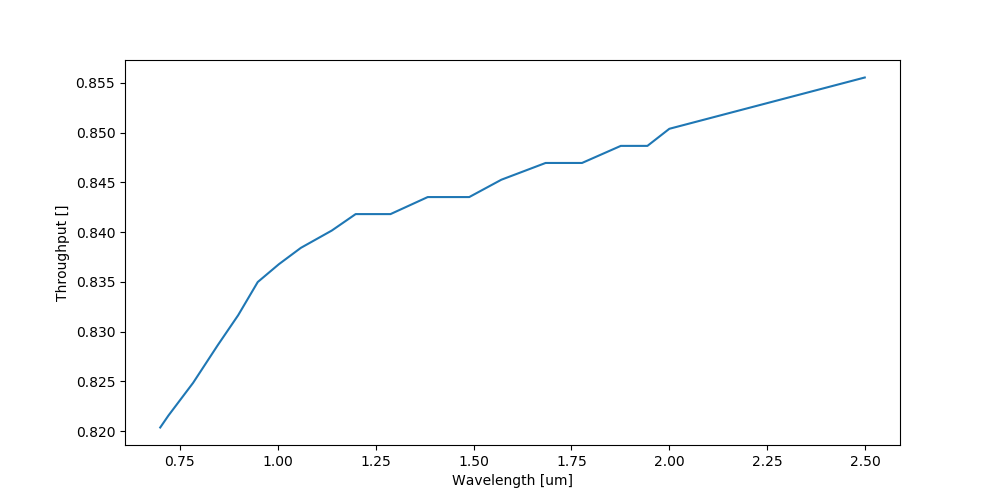
\includegraphics{maory_mms_ter.png}}\phantomsection\label{fig-maory-mms-ter}
\end{figure}


\paragraph{Meta-data%
  \label{meta-data}%
}

\begin{quote}
\begin{alltt}
\begin{lstlisting}[frame=single]
            filename : TER_MAORY_MMS.dat
                name : maory_mms_ter
                 psf : \{'strehl': 0.4, 'wavelength': 'Ks'\}
        element_name : MICADO_MCAO
              author : Auto-compiled from source
              source : LIST_mirrors_maory_mms.tbl
        date_created : 2020-08-25
       date_modified : 2020-08-25
                area : 0.9503317777109126
           area_unit : m2
     wavelength_unit : um
       emission_unit : photlam
             z_order : [10, 110, 510]
             include : True
        ignore_wings : False
            wave_min : 0.7
            wave_max : 2.5
           wave_unit : um
            wave_bin : 0.001
 report_plot_include : True
report_table_include : False
\end{lstlisting}
\end{alltt}
\end{quote}


\subsubsection{AnisocadoConstPSF: \textquotedbl{}maory\_const\_psf\textquotedbl{}%
  \label{anisocadoconstpsf-maory-const-psf}%
}

\textbf{Included by default}: \texttt{True}

\textbf{File Description}: field constant PSF as produced by MAORY

\textbf{Class Description}: Makes a SCAO on-axis PSF with a desired Strehl ratio at a given wavelength

\textbf{Changes}:

\begin{itemize}
\item \end{itemize}


\paragraph{Data%
  \label{id1}%
}

\begin{figure}[H]
\noindent\makebox[\linewidth][c]{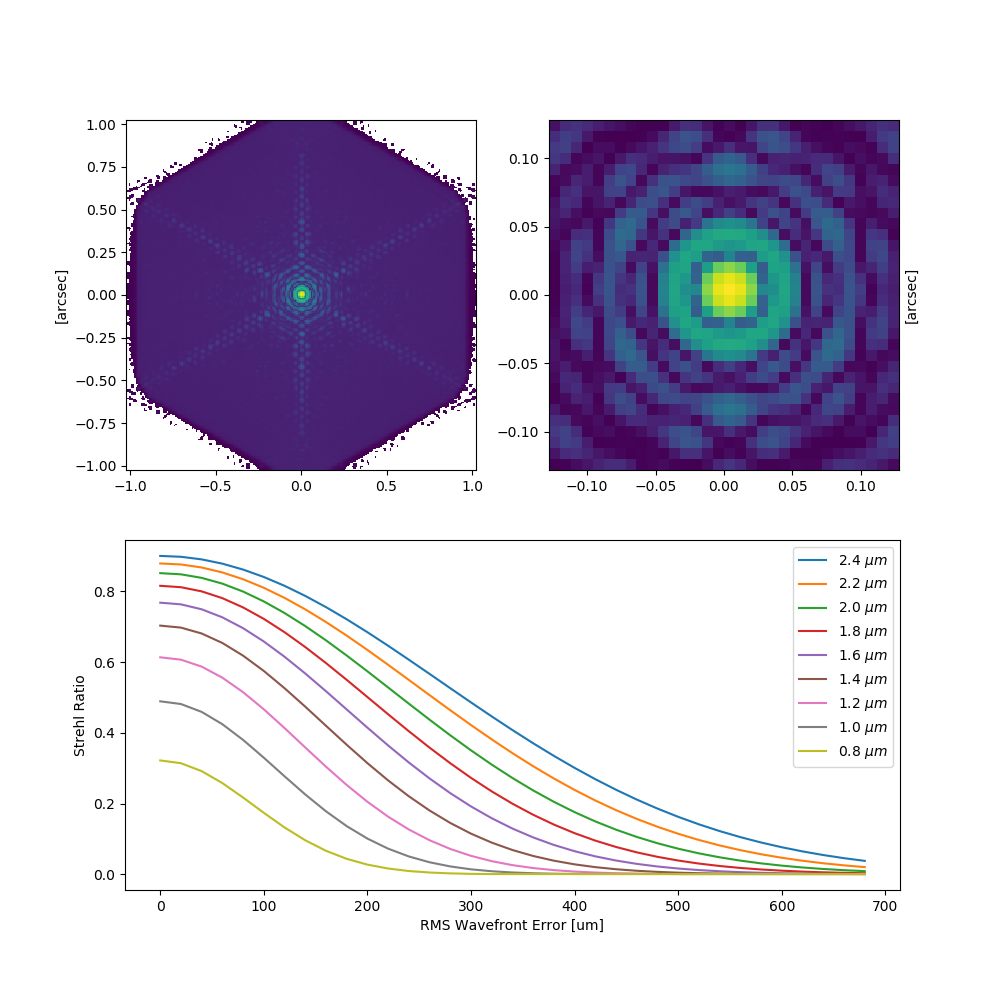
\includegraphics{maory_const_psf.png}}\phantomsection\label{fig-maory-const-psf}
\end{figure}


\paragraph{Meta-data%
  \label{id2}%
}

\begin{quote}
\begin{alltt}
\begin{lstlisting}[frame=single]
            filename : MICADO_AnisoCADO_rms_map.fits
                name : maory_const_psf
                 psf : \{'strehl': 0.4, 'wavelength': 'Ks'\}
        element_name : MICADO_MCAO
              strehl : !INST.psf.strehl
          wavelength : !INST.psf.wavelength
     psf_side_length : 256
              offset : [0, 0]
       rounded_edges : True
       convolve_mode : full
              SIMPLE : True
              BITPIX : -64
               NAXIS : 2
              NAXIS1 : 35
              NAXIS2 : 9
              EXTEND : True
              CRVAL1 : 0
              CRVAL2 : 0.8
              CRPIX1 : 1.0
              CRPIX2 : 1.0
              CDELT1 : 20
              CDELT2 : 0.2
              CUNIT1 : nm
              CUNIT2 : um
              CTYPE1 : LINEAR
              CTYPE2 : LINEAR
              LABEL1 : nmRMS
              LABEL2 : wavelength
              AUTHOR : Kieran Leschinski
            DATE_CRE : 2019-07-30
            DATE_MOD : 2019-07-30
              SOURCE : AnisoCADO
              STATUS : Strehl as a function of wavelength and wavefront error (nmRMS)
               ETYPE : SRMAP
                ECAT : -1
               EDATA : 0
             XOFFSET : 0
             YOFFSET : 0
             z_order : [42, 652]
             include : True
       flux_accuracy : 0.001
      sub_pixel_flag : False
            wave_key : WAVE0
    normalise_kernel : True
 report_plot_include : True
report_table_include : False
\end{lstlisting}
\end{alltt}
\end{quote}



\section{OpticalElement: \textquotedbl{}MICADO\_Sci\_MCAO\_detector\_override\textquotedbl{}%
  \label{opticalelement-micado-sci-mcao-detector-override}%
}

\textbf{Element}: detector

\textbf{Alias}: DET

\textbf{Description}: A settable window on the detector plane


\subsection{Global properties%
  \label{global-properties}%
}

\begin{quote}
\begin{alltt}
\begin{lstlisting}[frame=single]
       width : 4096
      height : 4096
element_name : MICADO_Sci_MCAO_detector_override
\end{lstlisting}
\end{alltt}
\end{quote}



\section{OpticalElement: \textquotedbl{}SPEC\textquotedbl{}%
  \label{opticalelement-spec}%
}

\textbf{Element}: instrument

\textbf{Alias}: INST

\textbf{Description}: Spectroscopy


\subsection{Global properties%
  \label{global-properties}%
}

\begin{quote}
\begin{alltt}
 filter_name : Spec_HK
 pixel_scale : 0.004
 plate_scale : 0.26666666666
element_name : SPEC
\end{alltt}
\end{quote}


\subsection{Effects%
  \label{effects}%
}

Summary of Effects included in this optical element:

\setlength{\DUtablewidth}{\linewidth}
\begin{longtable*}[c]{|p{0.098\DUtablewidth}|p{0.063\DUtablewidth}|p{0.075\DUtablewidth}|p{0.110\DUtablewidth}|p{0.110\DUtablewidth}|}
\hline
\textbf{%
element
} & \textbf{%
name
} & \textbf{%
class
} & \textbf{%
included
} & \textbf{%
z\_orders
} \\
\hline
\endfirsthead
\hline
\textbf{%
element
} & \textbf{%
name
} & \textbf{%
class
} & \textbf{%
included
} & \textbf{%
z\_orders
} \\
\hline
\endhead
\multicolumn{5}{c}{\hfill ... continued on next page} \\
\endfoot
\endlastfoot
 &  &  &  &  \\
\hline
\end{longtable*}
\label{tbl-spec}



\section{OpticalElement: \textquotedbl{}MICADO\_SPEC\textquotedbl{}%
  \label{opticalelement-micado-spec}%
}

\textbf{Element}: instrument

\textbf{Alias}: INST

\textbf{Description}: MICADO SPEC mode effects


\subsection{Global properties%
  \label{global-properties}%
}

\begin{quote}
\begin{alltt}
\begin{lstlisting}[frame=single]
         psf : \{'wavelength': '!INST.filter_name', 'strehl': 0.4\}
    aperture : \{'x': 0, 'y': 0, 'width': 3, 'height': 0.05\}
element_name : MICADO_SPEC
\end{lstlisting}
\end{alltt}
\end{quote}


\subsection{Effects%
  \label{effects}%
}

Summary of Effects included in this optical element:

\setlength{\DUtablewidth}{\linewidth}
\begin{longtable*}[c]{|p{0.135\DUtablewidth}|p{0.286\DUtablewidth}|p{0.265\DUtablewidth}|p{0.102\DUtablewidth}|p{0.167\DUtablewidth}|}
\hline
\textbf{%
element
} & \textbf{%
name
} & \textbf{%
class
} & \textbf{%
included
} & \textbf{%
z\_orders
} \\
\hline
\endfirsthead
\hline
\textbf{%
element
} & \textbf{%
name
} & \textbf{%
class
} & \textbf{%
included
} & \textbf{%
z\_orders
} \\
\hline
\endhead
\multicolumn{5}{c}{\hfill ... continued on next page} \\
\endfoot
\endlastfoot

MICADO\_SPEC
 & 
micado\_adjustable\_slit
 & 
RectangularApertureMask
 & 
True
 & 
{[}80, 280, 380{]}
 \\
\hline

MICADO\_SPEC
 & 
spectral\_trace\_3000x50mas
 & 
SpectralTraceList
 & 
True
 & 
{[}70, 270{]}
 \\
\hline
\end{longtable*}
\label{tbl-micado-spec}


\subsubsection{RectangularApertureMask: \textquotedbl{}micado\_adjustable\_slit\textquotedbl{}%
  \label{rectangularaperturemask-micado-adjustable-slit}%
}

\textbf{Included by default}: \texttt{True}

\textbf{File Description}:

\textbf{Class Description}: <no docstring>

\textbf{Changes}:

\begin{itemize}
\item \end{itemize}


\paragraph{Data%
  \label{data}%
}
\leavevmode
\setlength{\DUtablewidth}{\linewidth}
\begin{longtable*}[c]{|p{0.098\DUtablewidth}|p{0.098\DUtablewidth}|}
\hline
\textbf{%
x
} & \textbf{%
y
} \\
\hline
\endfirsthead
\hline
\textbf{%
x
} & \textbf{%
y
} \\
\hline
\endhead
\multicolumn{2}{c}{\hfill ... continued on next page} \\
\endfoot
\endlastfoot

-1.5000
 & 
-0.0250
 \\
\hline

1.5000
 & 
-0.0250
 \\
\hline

1.5000
 & 
0.0250
 \\
\hline

-1.5000
 & 
0.0250
 \\
\hline
\end{longtable*}
\label{tbl-micado-adjustable-slit}


\paragraph{Meta-data%
  \label{meta-data}%
}

\begin{quote}
\begin{alltt}
\begin{lstlisting}[frame=single]
             filename : None
                 name : micado_adjustable_slit
                  psf : \{'wavelength': 'Ks', 'strehl': 0.4\}
             aperture : \{'x': 0, 'y': 0, 'width': 3, 'height': 0.05\}
         element_name : MICADO_SPEC
                width : !INST.aperture.width
               height : !INST.aperture.height
                    x : !INST.aperture.x
                    y : !INST.aperture.y
              z_order : [80, 280, 380]
              include : True
          pixel_scale : !INST.pixel_scale
              no_mask : True
                angle : 0
                shape : rect
       conserve_image : True
                   id : 0
  report_plot_include : False
 report_table_include : True
report_table_rounding : 4
               x_unit : arcsec
               y_unit : arcsec
\end{lstlisting}
\end{alltt}
\end{quote}


\subsubsection{<SpectralTraceList> \textquotedbl{}spectral\_trace\_3000x50mas\textquotedbl{} : 1 traces%
  \label{spectraltracelist-spectral-trace-3000x50mas-1-traces}%
}

\textbf{Included by default}: \texttt{True}

\textbf{File Description}:

\textbf{Class Description}: List of spectral trace geometries for the detector plane

\textbf{Changes}:

\begin{itemize}
\item \end{itemize}


\paragraph{Data%
  \label{id1}%
}

\begin{figure}[H]
\noindent\makebox[\linewidth][c]{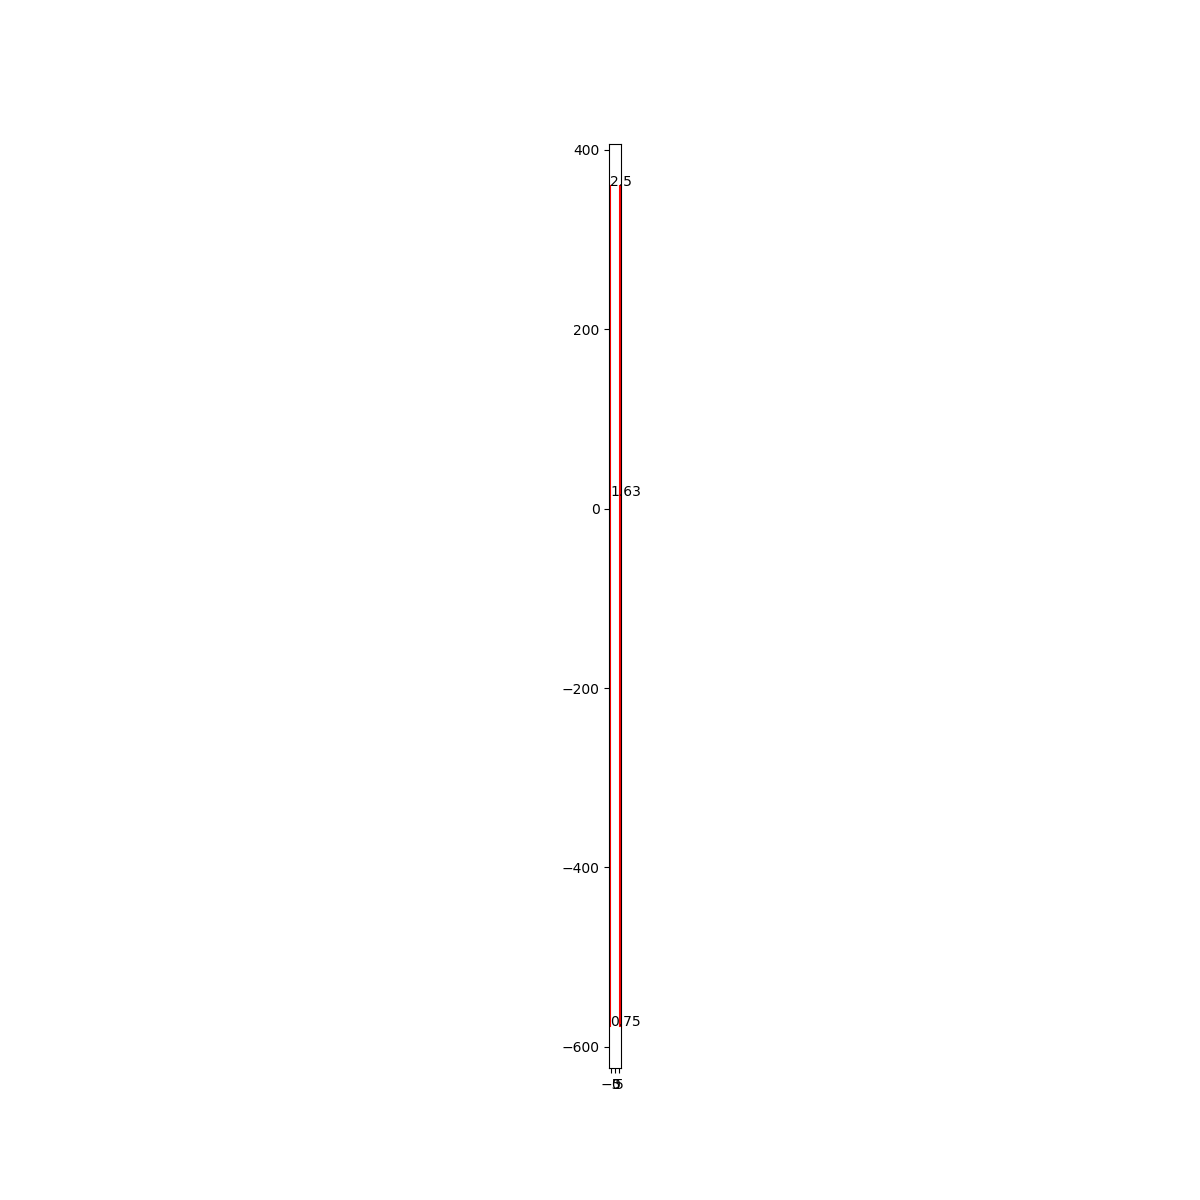
\includegraphics{spectral_trace_3000x50mas.png}}\phantomsection\label{fig-spectral-trace-3000x50mas}
\end{figure}


\paragraph{Meta-data%
  \label{id2}%
}

\begin{quote}
\begin{alltt}
\begin{lstlisting}[frame=single]
            filename : TRACE_SCI_3arcsec.fits
                name : spectral_trace_3000x50mas
                 psf : \{'wavelength': 'Ks', 'strehl': 0.4\}
            aperture : \{'x': 0, 'y': 0, 'width': 3, 'height': 0.05\}
        element_name : MICADO_SPEC
  center_on_wave_mid : True
              SIMPLE : True
              BITPIX : 8
               NAXIS : 0
              EXTEND : True
                ECAT : 1
               EDATA : 2
             z_order : [70, 270]
             include : True
         pixel_scale : !INST.pixel_scale
         plate_scale : !INST.plate_scale
            wave_min : !SIM.spectral.wave_min
            wave_mid : !SIM.spectral.wave_mid
            wave_max : !SIM.spectral.wave_max
           x_colname : x
           y_colname : y
           s_colname : s
        wave_colname : wavelength
    col_number_start : 0
               dwave : 0.002
       invalid_value : None
 report_plot_include : True
report_table_include : False
\end{lstlisting}
\end{alltt}
\end{quote}



\section{OpticalElement: \textquotedbl{}MICADO\_Sci\_SPEC\_detector\_override\textquotedbl{}%
  \label{opticalelement-micado-sci-spec-detector-override}%
}

\textbf{Element}: detector

\textbf{Alias}: DET

\textbf{Description}: A settable window on the detector plane


\subsection{Global properties%
  \label{global-properties}%
}

\begin{quote}
\begin{alltt}
\begin{lstlisting}[frame=single]
       width : 800
      height : 1024
element_name : MICADO_Sci_SPEC_detector_override
\end{lstlisting}
\end{alltt}
\end{quote}



\section{OpticalElement: \textquotedbl{}4mas\textquotedbl{}%
  \label{opticalelement-4mas}%
}

\textbf{Element}: instrument

\textbf{Alias}: INST

\textbf{Description}: wide-field imager  : 4mas/pix


\subsection{Global properties%
  \label{global-properties}%
}

\begin{quote}
\begin{alltt}
 filter_name : Ks
 pixel_scale : 0.004
 plate_scale : 0.26666666666
element_name : 4mas
\end{alltt}
\end{quote}


\subsection{Effects%
  \label{effects}%
}

Summary of Effects included in this optical element:

\setlength{\DUtablewidth}{\linewidth}
\begin{longtable*}[c]{|p{0.098\DUtablewidth}|p{0.063\DUtablewidth}|p{0.075\DUtablewidth}|p{0.110\DUtablewidth}|p{0.110\DUtablewidth}|}
\hline
\textbf{%
element
} & \textbf{%
name
} & \textbf{%
class
} & \textbf{%
included
} & \textbf{%
z\_orders
} \\
\hline
\endfirsthead
\hline
\textbf{%
element
} & \textbf{%
name
} & \textbf{%
class
} & \textbf{%
included
} & \textbf{%
z\_orders
} \\
\hline
\endhead
\multicolumn{5}{c}{\hfill ... continued on next page} \\
\endfoot
\endlastfoot
 &  &  &  &  \\
\hline
\end{longtable*}
\label{tbl-4mas}



\section{OpticalElement: \textquotedbl{}1.5mas\textquotedbl{}%
  \label{opticalelement-1-5mas}%
}

\textbf{Element}: instrument

\textbf{Alias}: INST

\textbf{Description}: zoom imager : 1.5mas/pix


\subsection{Global properties%
  \label{global-properties}%
}

\begin{quote}
\begin{alltt}
\begin{lstlisting}[frame=single]
 filter_name : Ks
 pixel_scale : 0.0015
 plate_scale : 0.1
element_name : 1.5mas
\end{lstlisting}
\end{alltt}
\end{quote}


\subsection{Effects%
  \label{effects}%
}

Summary of Effects included in this optical element:

\setlength{\DUtablewidth}{\linewidth}
\begin{longtable*}[c]{|p{0.098\DUtablewidth}|p{0.063\DUtablewidth}|p{0.075\DUtablewidth}|p{0.110\DUtablewidth}|p{0.110\DUtablewidth}|}
\hline
\textbf{%
element
} & \textbf{%
name
} & \textbf{%
class
} & \textbf{%
included
} & \textbf{%
z\_orders
} \\
\hline
\endfirsthead
\hline
\textbf{%
element
} & \textbf{%
name
} & \textbf{%
class
} & \textbf{%
included
} & \textbf{%
z\_orders
} \\
\hline
\endhead
\multicolumn{5}{c}{\hfill ... continued on next page} \\
\endfoot
\endlastfoot
 &  &  &  &  \\
\hline
\end{longtable*}
\label{tbl-1-5mas}



\section{OpticalElement: \textquotedbl{}micado\_sci\_detector\textquotedbl{}%
  \label{opticalelement-micado-sci-detector}%
}

\textbf{Element}: detector

\textbf{Alias}: DET

\textbf{Description}: List of MICADO detector effects relevant for astronomers


\subsection{Global properties%
  \label{global-properties}%
}

\begin{quote}
\begin{alltt}
\begin{lstlisting}[frame=single]
image_plane_id : 0
   temperature : -230
           dit : !OBS.dit
          ndit : !OBS.ndit
         width : 4096
        height : 4096
             x : 0
             y : 0
  element_name : micado_sci_detector
\end{lstlisting}
\end{alltt}
\end{quote}


\subsection{Effects%
  \label{effects}%
}

Summary of Effects included in this optical element:

\setlength{\DUtablewidth}{\linewidth}
\begin{longtable*}[c]{|p{0.195\DUtablewidth}|p{0.233\DUtablewidth}|p{0.242\DUtablewidth}|p{0.090\DUtablewidth}|p{0.195\DUtablewidth}|}
\hline
\textbf{%
element
} & \textbf{%
name
} & \textbf{%
class
} & \textbf{%
included
} & \textbf{%
z\_orders
} \\
\hline
\endfirsthead
\hline
\textbf{%
element
} & \textbf{%
name
} & \textbf{%
class
} & \textbf{%
included
} & \textbf{%
z\_orders
} \\
\hline
\endhead
\multicolumn{5}{c}{\hfill ... continued on next page} \\
\endfoot
\endlastfoot

micado\_sci\_detector
 & 
micado\_detector\_window
 & 
DetectorWindow
 & 
True
 & 
{[}90, 290, 390, 490{]}
 \\
\hline

micado\_sci\_detector
 & 
h4rg\_qe\_curve
 & 
QuantumEfficiencyCurve
 & 
True
 & 
{[}113, 513{]}
 \\
\hline

micado\_sci\_detector
 & 
exposure\_action
 & 
SummedExposure
 & 
True
 & 
{[}860{]}
 \\
\hline

micado\_sci\_detector
 & 
dark\_current
 & 
DarkCurrent
 & 
True
 & 
{[}830{]}
 \\
\hline

micado\_sci\_detector
 & 
shot\_noise
 & 
ShotNoise
 & 
True
 & 
{[}820{]}
 \\
\hline

micado\_sci\_detector
 & 
h4rg\_detector\_linearity
 & 
LinearityCurve
 & 
False
 & 
{[}840{]}
 \\
\hline

micado\_sci\_detector
 & 
readout\_noise
 & 
PoorMansHxRGReadoutNoise
 & 
True
 & 
{[}811{]}
 \\
\hline
\end{longtable*}
\label{tbl-micado-sci-detector}


\subsubsection{DetectorWindow: \textquotedbl{}micado\_detector\_window\textquotedbl{}%
  \label{detectorwindow-micado-detector-window}%
}

\textbf{Included by default}: \texttt{True}

\textbf{File Description}:

\textbf{Class Description}: For when a full DetectorList if too cumbersome

\textbf{Changes}:

\begin{itemize}
\item \end{itemize}


\paragraph{Data%
  \label{data}%
}

\begin{figure}[H]
\noindent\makebox[\linewidth][c]{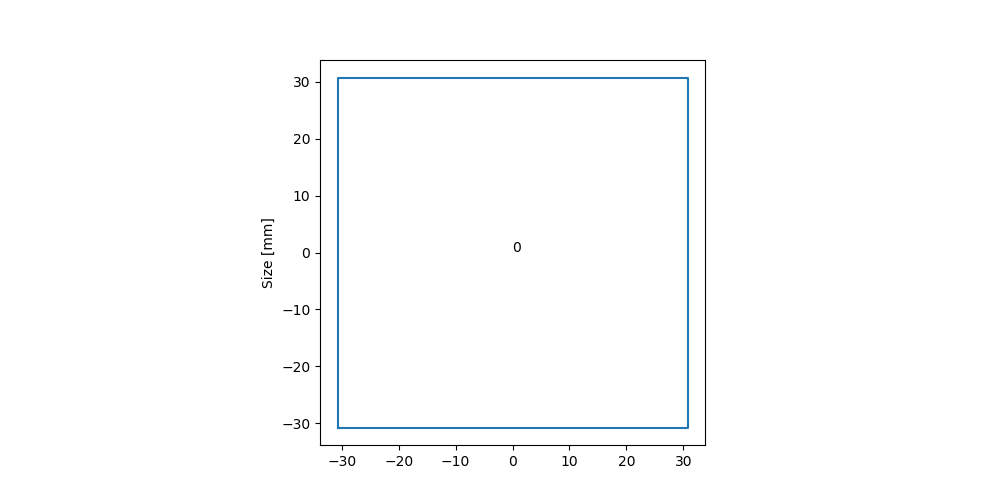
\includegraphics{micado_detector_window.png}}\phantomsection\label{fig-micado-detector-window}
\end{figure}

\setlength{\DUtablewidth}{\linewidth}
\begin{longtable*}[c]{|p{0.051\DUtablewidth}|p{0.086\DUtablewidth}|p{0.086\DUtablewidth}|p{0.133\DUtablewidth}|p{0.145\DUtablewidth}|p{0.075\DUtablewidth}|p{0.063\DUtablewidth}|p{0.133\DUtablewidth}|}
\hline
\textbf{%
id
} & \textbf{%
x\_cen
} & \textbf{%
y\_cen
} & \textbf{%
x\_size
} & \textbf{%
y\_size
} & \textbf{%
angle
} & \textbf{%
gain
} & \textbf{%
pixel\_size
} \\
\hline
\endfirsthead
\hline
\textbf{%
id
} & \textbf{%
x\_cen
} & \textbf{%
y\_cen
} & \textbf{%
x\_size
} & \textbf{%
y\_size
} & \textbf{%
angle
} & \textbf{%
gain
} & \textbf{%
pixel\_size
} \\
\hline
\endhead
\multicolumn{8}{c}{\hfill ... continued on next page} \\
\endfoot
\endlastfoot

0
 & 
!DET.x
 & 
!DET.y
 & 
!DET.width
 & 
!DET.height
 & 
0
 & 
1
 & 
0.015
 \\
\hline
\end{longtable*}
\label{tbl-micado-detector-window}


\paragraph{Meta-data%
  \label{meta-data}%
}

\begin{quote}
\begin{alltt}
\begin{lstlisting}[frame=single]
            filename : None
                name : micado_detector_window
          orig_units : pixel
          x_cen_unit : pixel
          y_cen_unit : pixel
         x_size_unit : pixel
         y_size_unit : pixel
     pixel_size_unit : mm
          angle_unit : deg
           gain_unit : electron/adu
      image_plane_id : 0
         temperature : -230
                 dit : !OBS.dit
                ndit : !OBS.ndit
        element_name : micado_sci_detector
             z_order : [90, 290, 390, 490]
             include : True
         pixel_scale : !INST.pixel_scale
    active_detectors : all
 report_plot_include : True
report_table_include : True
\end{lstlisting}
\end{alltt}
\end{quote}


\subsubsection{QuantumEfficiencyCurve: \textquotedbl{}h4rg\_qe\_curve\textquotedbl{}%
  \label{quantumefficiencycurve-h4rg-qe-curve}%
}

\textbf{Included by default}: \texttt{True}

\textbf{File Description}: Quantum efficiency curves for each detector

\textbf{Class Description}: <no docstring>

\textbf{Changes}:

\begin{itemize}
\item 2018-11-19 (KL) updated meta data to new format

\item 2019-08-09 (KL) Added action keyword to meta data
\end{itemize}


\paragraph{Data%
  \label{id1}%
}

\begin{figure}[H]
\noindent\makebox[\linewidth][c]{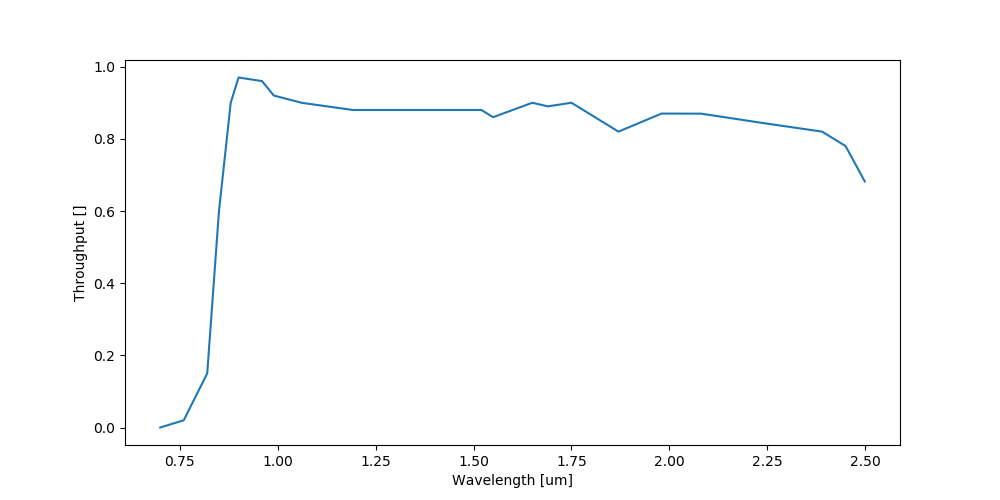
\includegraphics{h4rg_qe_curve.png}}\phantomsection\label{fig-h4rg-qe-curve}
\end{figure}


\paragraph{Meta-data%
  \label{id2}%
}

\begin{quote}
\begin{alltt}
\begin{lstlisting}[frame=single]
            filename : QE_detector_H2RG.dat
                name : h4rg_qe_curve
      image_plane_id : 0
         temperature : -230
                 dit : 60
                ndit : 1
               width : 4096
              height : 4096
                   x : 0
                   y : 0
        element_name : micado_sci_detector
              author : Kieran Leschinski
             sources : Finger+ 2008 SPIE
        date_created : 2016-01-01
       date_modified : 2019-08-09
                type : detector:quantum_efficiency
              status : Design, guestimated by reading off the graph in Finger+ 2008
     wavelength_unit : um
              action : transmission
             z_order : [113, 513]
             include : True
        ignore_wings : False
            wave_min : 0.7
            wave_max : 2.5
           wave_unit : um
            wave_bin : 0.001
 report_plot_include : True
report_table_include : False
            position : -1
\end{lstlisting}
\end{alltt}
\end{quote}


\subsubsection{SummedExposure: \textquotedbl{}exposure\_action\textquotedbl{}%
  \label{summedexposure-exposure-action}%
}

\textbf{Included by default}: \texttt{True}

\textbf{File Description}: Summing up sky signal for all DITs and NDITs

\textbf{Class Description}: Simulates a summed stack of \texttt{ndit} exposures

\textbf{Changes}:

\begin{itemize}
\item \end{itemize}


\paragraph{Data%
  \label{id3}%
}


\paragraph{Meta-data%
  \label{id4}%
}

\begin{quote}
\begin{alltt}
\begin{lstlisting}[frame=single]
      filename : None
          name : exposure_action
image_plane_id : 0
   temperature : -230
           dit : !OBS.dit
          ndit : !OBS.ndit
         width : 4096
        height : 4096
             x : 0
             y : 0
  element_name : micado_sci_detector
       z_order : [860]
       include : True
\end{lstlisting}
\end{alltt}
\end{quote}


\subsubsection{DarkCurrent: \textquotedbl{}dark\_current\textquotedbl{}%
  \label{darkcurrent-dark-current}%
}

\textbf{Included by default}: \texttt{True}

\textbf{File Description}: MICADO dark current

\textbf{Class Description}: required: dit, ndit, value

\textbf{Changes}:

\begin{itemize}
\item \end{itemize}


\paragraph{Data%
  \label{id5}%
}


\paragraph{Meta-data%
  \label{id6}%
}

\begin{quote}
\begin{alltt}
\begin{lstlisting}[frame=single]
      filename : None
          name : dark_current
image_plane_id : 0
   temperature : -230
           dit : !OBS.dit
          ndit : !OBS.ndit
         width : 4096
        height : 4096
             x : 0
             y : 0
  element_name : micado_sci_detector
         value : 0.1
       z_order : [830]
       include : True
\end{lstlisting}
\end{alltt}
\end{quote}


\subsubsection{ShotNoise: \textquotedbl{}shot\_noise\textquotedbl{}%
  \label{shotnoise-shot-noise}%
}

\textbf{Included by default}: \texttt{True}

\textbf{File Description}: apply poisson shot noise to images

\textbf{Class Description}: <no docstring>

\textbf{Changes}:

\begin{itemize}
\item \end{itemize}


\paragraph{Data%
  \label{id7}%
}


\paragraph{Meta-data%
  \label{id8}%
}

\begin{quote}
\begin{alltt}
\begin{lstlisting}[frame=single]
      filename : None
          name : shot_noise
image_plane_id : 0
   temperature : -230
           dit : !OBS.dit
          ndit : !OBS.ndit
         width : 4096
        height : 4096
             x : 0
             y : 0
  element_name : micado_sci_detector
       z_order : [820]
       include : True
   random_seed : !SIM.random.seed
\end{lstlisting}
\end{alltt}
\end{quote}


\subsubsection{LinearityCurve: \textquotedbl{}h4rg\_detector\_linearity\textquotedbl{}%
  \label{linearitycurve-h4rg-detector-linearity}%
}

\textbf{Included by default}: \texttt{False}

\textbf{File Description}: Linearity characteristics of H4RG chips

\textbf{Class Description}: <no docstring>

\textbf{Changes}:

\begin{itemize}
\item 2018-11-19 (KL) updated meta data to new format

\item 2019-08-14 (KL) replaced long 1000000000 with 1e99
\end{itemize}


\paragraph{Data%
  \label{id9}%
}

\begin{figure}[H]
\noindent\makebox[\linewidth][c]{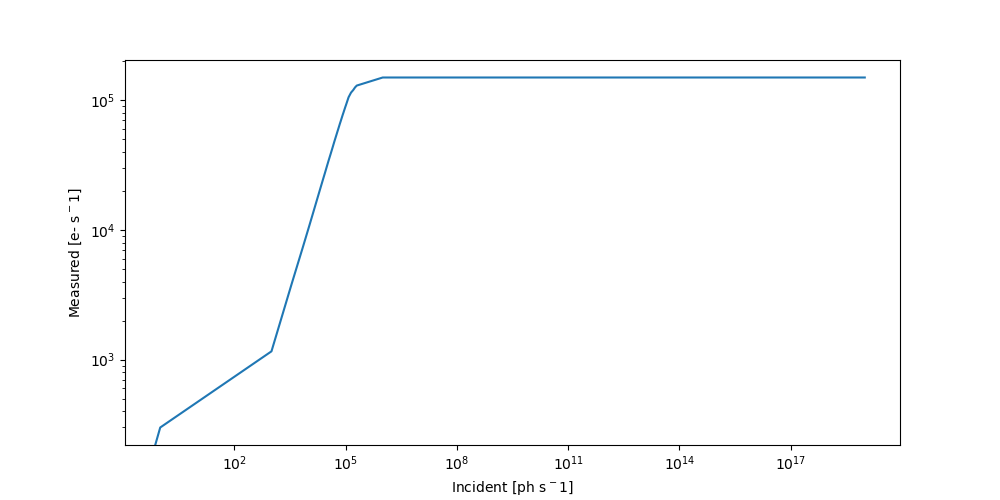
\includegraphics{h4rg_detector_linearity.png}}\phantomsection\label{fig-h4rg-detector-linearity}
\end{figure}


\paragraph{Meta-data%
  \label{id10}%
}

\begin{quote}
\begin{alltt}
\begin{lstlisting}[frame=single]
            filename : FPA_linearity.dat
                name : h4rg_detector_linearity
             include : False
      image_plane_id : 0
         temperature : -230
                 dit : !OBS.dit
                ndit : !OBS.ndit
               width : 4096
              height : 4096
                   x : 0
                   y : 0
        element_name : micado_sci_detector
              author : Kieran Leschinski
             sources : Ingraham+ 2014 - Gemini Calibrations II for H2RG
        date_created : 2016-01-01
       date_modified : 2018-11-19
                type : detector:linearity
              status : Design, approximated from the H2RG
       incident_unit : ph
       measured_unit : ph
             z_order : [840]
 report_plot_include : True
report_table_include : False
\end{lstlisting}
\end{alltt}
\end{quote}


\subsubsection{PoorMansHxRGReadoutNoise: \textquotedbl{}readout\_noise\textquotedbl{}%
  \label{poormanshxrgreadoutnoise-readout-noise}%
}

\textbf{Included by default}: \texttt{True}

\textbf{File Description}: Readout noise frames

\textbf{Class Description}: <no docstring>

\textbf{Changes}:

\begin{itemize}
\item \end{itemize}


\paragraph{Data%
  \label{id11}%
}


\paragraph{Meta-data%
  \label{id12}%
}

\begin{quote}
\begin{alltt}
\begin{lstlisting}[frame=single]
            filename : None
                name : readout_noise
      image_plane_id : 0
         temperature : -230
                 dit : !OBS.dit
                ndit : !OBS.ndit
               width : 4096
              height : 4096
                   x : 0
                   y : 0
        element_name : micado_sci_detector
           noise_std : 12
          n_channels : 64
             z_order : [811]
             include : True
   pedestal_fraction : 0.3
       read_fraction : 0.4
       line_fraction : 0.25
    channel_fraction : 0.05
         random_seed : !SIM.random.seed
 report_plot_include : False
report_table_include : False
\end{lstlisting}
\end{alltt}
\end{quote}

\end{samepage}

\chapter{Supoort packages}

\begin{samepage}


\section{OpticalElement: \textquotedbl{}armazones\textquotedbl{}%
  \label{opticalelement-armazones}%
}

\textbf{Element}: atmosphere

\textbf{Alias}: ATMO

\textbf{Description}: Atmosphere and location details for Cerro Armazones


\subsection{Global properties%
  \label{global-properties}%
}

\begin{quote}
\begin{alltt}
\begin{lstlisting}[frame=single]
    altitude : 3060
   longitude : -70.1918
    latitude : -24.5899
 temperature : 7
    humidity : 0.1
    pressure : 0.755
         pwv : 2.5
     airmass : !OBS.airmass
 pupil_angle : !OBS.pupil_angle
 pixel_scale : !INST.pixel_scale
element_name : armazones
\end{lstlisting}
\end{alltt}
\end{quote}


\subsection{Effects%
  \label{effects}%
}

Summary of Effects included in this optical element:

\setlength{\DUtablewidth}{\linewidth}
\begin{longtable*}[c]{|p{0.114\DUtablewidth}|p{0.366\DUtablewidth}|p{0.246\DUtablewidth}|p{0.103\DUtablewidth}|p{0.125\DUtablewidth}|}
\hline
\textbf{%
element
} & \textbf{%
name
} & \textbf{%
class
} & \textbf{%
included
} & \textbf{%
z\_orders
} \\
\hline
\endfirsthead
\hline
\textbf{%
element
} & \textbf{%
name
} & \textbf{%
class
} & \textbf{%
included
} & \textbf{%
z\_orders
} \\
\hline
\endhead
\multicolumn{5}{c}{\hfill ... continued on next page} \\
\endfoot
\endlastfoot

armazones
 & 
armazones\_atmo\_default\_ter\_curve
 & 
AtmosphericTERCurve
 & 
True
 & 
{[}111, 511{]}
 \\
\hline

armazones
 & 
armazones\_atmo\_dispersion
 & 
AtmosphericDispersion
 & 
True
 & 
{[}231{]}
 \\
\hline

armazones
 & 
armazones\_atmo\_skycalc\_ter\_curve
 & 
SkycalcTERCurve
 & 
False
 & 
{[}112, 512{]}
 \\
\hline
\end{longtable*}
\label{tbl-armazones}


\subsubsection{AtmosphericTERCurve: \textquotedbl{}armazones\_atmo\_default\_ter\_curve\textquotedbl{}%
  \label{atmospherictercurve-armazones-atmo-default-ter-curve}%
}

\textbf{Included by default}: \texttt{True}

\textbf{File Description}: atmospheric emission and transmission

\textbf{Class Description}: <no docstring>

\textbf{Changes}:

\begin{itemize}
\item 2019-07-24 (KL) Created file

\item 2019-08-09 (KL) Updated values for airmass 1.2, pwv 2.5
\end{itemize}


\paragraph{Data%
  \label{data}%
}


\paragraph{Meta-data%
  \label{meta-data}%
}

\begin{quote}
\begin{alltt}
\begin{lstlisting}[frame=single]
       filename : TER_armazones_default_NIR_IMG.dat
           name : armazones_atmo_default_ter_curve
        include : True
       altitude : 3060
      longitude : -70.1918
       latitude : -24.5899
    temperature : 7
       humidity : 0.1
       pressure : 0.755
            pwv : 2.5
        airmass : !OBS.airmass
    pupil_angle : !OBS.pupil_angle
    pixel_scale : !INST.pixel_scale
   element_name : armazones
         author : Kieran Leschinski
         source : skycalc website for standard Armazones conditions
   date_created : 2019-07-24
  date_modified : 2019-08-09
         status : Design
           type : atmosphere:ter_curve
         season : entire year
           time : entire night
         action : transmission
wavelength_unit : um
  emission_unit : ph s-1 m-2 um-1 arcsec-2
        z_order : [111, 511]
   ignore_wings : False
       wave_min : !SIM.spectral.wave_min
       wave_max : !SIM.spectral.wave_max
      wave_unit : !SIM.spectral.wave_unit
       wave_bin : !SIM.spectral.spectral_resolution
           area : !TEL.area
      area_unit : m2
       position : 0
\end{lstlisting}
\end{alltt}
\end{quote}


\subsubsection{AtmosphericDispersion: \textquotedbl{}armazones\_atmo\_dispersion\textquotedbl{}%
  \label{atmosphericdispersion-armazones-atmo-dispersion}%
}

\textbf{Included by default}: \texttt{True}

\textbf{File Description}: atmospheric dispersion

\textbf{Class Description}: Used to generate the wavelength bins based on shifts due to the atmosphere

\textbf{Changes}:

\begin{itemize}
\item \end{itemize}


\paragraph{Data%
  \label{id1}%
}


\paragraph{Meta-data%
  \label{id2}%
}

\begin{quote}
\begin{alltt}
\begin{lstlisting}[frame=single]
          filename : None
              name : armazones_atmo_dispersion
          altitude : 3060
         longitude : -70.1918
          latitude : -24.5899
       temperature : 7
          humidity : 0.1
          pressure : 0.755
               pwv : 2.5
           airmass : !OBS.airmass
       pupil_angle : !OBS.pupil_angle
       pixel_scale : !INST.pixel_scale
      element_name : armazones
           z_order : [231]
           include : True
          wave_min : !SIM.spectral.wave_min
          wave_mid : !SIM.spectral.wave_mid
          wave_max : !SIM.spectral.wave_max
sub_pixel_fraction : !SIM.sub_pixel.fraction
         num_steps : 1000
\end{lstlisting}
\end{alltt}
\end{quote}


\subsubsection{SkycalcTERCurve: \textquotedbl{}armazones\_atmo\_skycalc\_ter\_curve\textquotedbl{}%
  \label{skycalctercurve-armazones-atmo-skycalc-ter-curve}%
}

\textbf{Included by default}: \texttt{False}

\textbf{File Description}: atmospheric spectra pulled from the skycalc server

\textbf{Class Description}: <no docstring>

\textbf{Changes}:

\begin{itemize}
\item \end{itemize}


\paragraph{Data%
  \label{id3}%
}


\paragraph{Meta-data%
  \label{id4}%
}

\begin{quote}
\begin{alltt}
\begin{lstlisting}[frame=single]
    filename : None
        name : armazones_atmo_skycalc_ter_curve
     include : False
    altitude : 3060
   longitude : -70.1918
    latitude : -24.5899
 temperature : 7
    humidity : 0.1
    pressure : 0.755
         pwv : 2.5
     airmass : !OBS.airmass
 pupil_angle : !OBS.pupil_angle
 pixel_scale : !INST.pixel_scale
element_name : armazones
 observatory : armazones
        wmin : 699.9999999999999
        wmax : 2499.9999999999995
       wunit : um
      wdelta : 0.09999999999999999
     z_order : [112, 512]
ignore_wings : False
    wave_min : !SIM.spectral.wave_min
    wave_max : !SIM.spectral.wave_max
   wave_unit : !SIM.spectral.wave_unit
    wave_bin : !SIM.spectral.spectral_resolution
      action : transmission
        area : !TEL.area
   area_unit : m2
    position : 0
\end{lstlisting}
\end{alltt}
\end{quote}



\section{OpticalElement: \textquotedbl{}ELT\textquotedbl{}%
  \label{opticalelement-elt}%
}

\textbf{Element}: telescope

\textbf{Alias}: TEL

\textbf{Description}: The extremely large telescope


\subsection{Global properties%
  \label{global-properties}%
}

\begin{quote}
\begin{alltt}
 temperature : !ATMO.temperature
element_name : ELT
\end{alltt}
\end{quote}


\subsection{Effects%
  \label{effects}%
}

Summary of Effects included in this optical element:

\setlength{\DUtablewidth}{\linewidth}
\begin{longtable*}[c]{|p{0.098\DUtablewidth}|p{0.284\DUtablewidth}|p{0.145\DUtablewidth}|p{0.110\DUtablewidth}|p{0.179\DUtablewidth}|}
\hline
\textbf{%
element
} & \textbf{%
name
} & \textbf{%
class
} & \textbf{%
included
} & \textbf{%
z\_orders
} \\
\hline
\endfirsthead
\hline
\textbf{%
element
} & \textbf{%
name
} & \textbf{%
class
} & \textbf{%
included
} & \textbf{%
z\_orders
} \\
\hline
\endhead
\multicolumn{5}{c}{\hfill ... continued on next page} \\
\endfoot
\endlastfoot

ELT
 & 
scope\_surface\_list
 & 
SurfaceList
 & 
True
 & 
{[}20, 120, 520{]}
 \\
\hline

ELT
 & 
scope\_vibration
 & 
Vibration
 & 
True
 & 
{[}244, 744{]}
 \\
\hline

ELT
 & 
eso\_combined\_reflection
 & 
TERCurve
 & 
False
 & 
{[}10, 110, 510{]}
 \\
\hline
\end{longtable*}
\label{tbl-elt}


\subsubsection{SurfaceList: \textquotedbl{}scope\_surface\_list\textquotedbl{}%
  \label{surfacelist-scope-surface-list}%
}

\textbf{Included by default}: \texttt{True}

\textbf{File Description}: list of ELT surfaces

\textbf{Class Description}: <no docstring>

\textbf{Changes}:

\begin{itemize}
\item 2018-11-19 (KL) Added meta data, added Action column

\item 2019-01-28 (KL) Fixed YAML format in meta data

\item 2020-08-17 (KL) Updated M1 and M4 dimensions according to ESO-253082\_4 sect 4.7 \textquotedbl{}all-glass\textquotedbl{} diameter

\item 2020-08-17 (KL) Pegged temperature to the atmosphere
\end{itemize}


\paragraph{Data%
  \label{data}%
}


\paragraph{Meta-data%
  \label{meta-data}%
}

\begin{quote}
\begin{alltt}
          filename : LIST_mirrors_ELT.tbl
              name : scope_surface_list
       temperature : !ATMO.temperature
      element_name : ELT
            author : Oliver Czoske, Kieran Leschinski
            source : ESO ELT DRM, ESO-253082_4
      date_created : 2018-11-19
     date_modified : 2020-08-17
            status : Design - pre MICADO-FDR mirror list
        outer_unit : m
        inner_unit : m
        angle_unit : degree
  temperature_unit : deg_C
             notes : ['2020-08-17 (KL) Coatings match those described in ESO-253082_4']
           z_order : [20, 120, 520]
           include : True
      ignore_wings : False
          wave_min : !SIM.spectral.wave_min
          wave_max : !SIM.spectral.wave_max
         wave_unit : !SIM.spectral.wave_unit
          wave_bin : !SIM.spectral.spectral_resolution
minimum_throughput : !SIM.spectral.minimum_throughput
           etendue : !TEL.etendue
\end{alltt}
\end{quote}


\subsubsection{Vibration: \textquotedbl{}scope\_vibration\textquotedbl{}%
  \label{vibration-scope-vibration}%
}

\textbf{Included by default}: \texttt{True}

\textbf{File Description}: residual vibration of telescope

\textbf{Class Description}: Creates a wavelength independent kernel image

\textbf{Changes}:

\begin{itemize}
\item \end{itemize}


\paragraph{Data%
  \label{id1}%
}


\paragraph{Meta-data%
  \label{id2}%
}

\begin{quote}
\begin{alltt}
        filename : None
            name : scope_vibration
     temperature : 7
    element_name : ELT
            fwhm : 0.001
     pixel_scale : 0.004
         z_order : [244, 744]
         include : True
   flux_accuracy : 0.001
  sub_pixel_flag : False
   convolve_mode : full
        wave_key : WAVE0
normalise_kernel : True
   width_n_fwhms : 4
\end{alltt}
\end{quote}


\subsubsection{TERCurve: \textquotedbl{}eso\_combined\_reflection\textquotedbl{}%
  \label{tercurve-eso-combined-reflection}%
}

\textbf{Included by default}: \texttt{False}

\textbf{File Description}: single combined reflection curve for clean ELT 5 mirror combination

\textbf{Class Description}: Transmission, Emissivity, Reflection Curve

\textbf{Changes}:

\begin{itemize}
\item 2019-11-06 (KL) Converted from .xlsx to .dat file, added ScopeSim meta data

\item 2020-07-09 (KL) Added inner and outer dimensions to meta, for use with MICADO-Sci

\item 2020-08-17 (KL) Added emissivity column according to ESO-253082\_4, sect 4.12.2
\end{itemize}


\paragraph{Data%
  \label{id3}%
}


\paragraph{Meta-data%
  \label{id4}%
}

\begin{quote}
\begin{alltt}
       filename : TER_ELT_system_20190611.dat
           name : eso_combined_reflection
        include : False
    temperature : !ATMO.temperature
   element_name : ELT
     temperture : !ATMO.temperature
         author : R. Holzloehner
         source : See ESO-306070 and ESO-293390 for background.
   date_created : 2018-09-18
  date_modified : 2019-06-11
           type : TERCurve
         status : design
         action : reflection
          outer : 37.3
     outer_unit : m
          inner : 11.1
     inner_unit : m
wavelength_unit : um
          notes : ['Baseline coatings.', 'Fresh coatings without contamination.', '4nm roughness modeled.', 'Partly based on measured data by Tom Schneider (Gemini).', 'Reflection is for the combined M1-M5 system, not for individual mirrors', 'Emissivity is calculated from ESO-253082_4, sect 4.12.2']
        z_order : [10, 110, 510]
   ignore_wings : False
       wave_min : !SIM.spectral.wave_min
       wave_max : !SIM.spectral.wave_max
      wave_unit : !SIM.spectral.wave_unit
       wave_bin : !SIM.spectral.spectral_resolution
\end{alltt}
\end{quote}



\section{OpticalElement: \textquotedbl{}MAORY\textquotedbl{}%
  \label{opticalelement-maory}%
}

\textbf{Element}: relay\_optics

\textbf{Alias}: RO

\textbf{Description}: MAORY AO relay module


\subsection{Global properties%
  \label{global-properties}%
}

\begin{quote}
\begin{alltt}
 temperature : !ATMO.temperature
psf_filename : None
element_name : MAORY
\end{alltt}
\end{quote}


\subsection{Effects%
  \label{effects}%
}

Summary of Effects included in this optical element:

\setlength{\DUtablewidth}{\linewidth}
\begin{longtable*}[c]{|p{0.098\DUtablewidth}|p{0.226\DUtablewidth}|p{0.203\DUtablewidth}|p{0.110\DUtablewidth}|p{0.179\DUtablewidth}|}
\hline
\textbf{%
element
} & \textbf{%
name
} & \textbf{%
class
} & \textbf{%
included
} & \textbf{%
z\_orders
} \\
\hline
\endfirsthead
\hline
\textbf{%
element
} & \textbf{%
name
} & \textbf{%
class
} & \textbf{%
included
} & \textbf{%
z\_orders
} \\
\hline
\endhead
\multicolumn{5}{c}{\hfill ... continued on next page} \\
\endfoot
\endlastfoot

MAORY
 & 
maory\_surface\_list
 & 
SurfaceList
 & 
True
 & 
{[}20, 120, 520{]}
 \\
\hline

MAORY
 & 
maory\_generic\_psf
 & 
FieldConstantPSF
 & 
True
 & 
{[}262, 662{]}
 \\
\hline
\end{longtable*}
\label{tbl-maory}


\subsubsection{SurfaceList: \textquotedbl{}maory\_surface\_list\textquotedbl{}%
  \label{surfacelist-maory-surface-list}%
}

\textbf{Included by default}: \texttt{True}

\textbf{File Description}: list of surfaces in MAORY

\textbf{Class Description}: <no docstring>

\textbf{Changes}:

\begin{itemize}
\item 2018-11-19 (KL) Added meta data, changed Dichr. filename

\item 2019-01-28 (KL) Fixed YAML format in meta data

\item 2020-06-22 (KL) Obsolete. Use LIST\_mirrors\_maory\_mms.tbl from now on.
\end{itemize}


\paragraph{Data%
  \label{data}%
}


\paragraph{Meta-data%
  \label{meta-data}%
}

\begin{quote}
\begin{alltt}
          filename : LIST_mirrors_MCAO_MAORY.tbl
              name : maory_surface_list
       temperature : !ATMO.temperature
      psf_filename : None
      element_name : MAORY
            author : Kieran Leschinski
            source : Ciliegi+ 2018 SPIE, "MAORY for ELT - preliminary design overview"
      date_created : 2018-11-19
     date_modified : 2018-11-19
            status : Design - pre PDR list of MAORY mirrors
              type : mirror:list
        outer_unit : m
        inner_unit : m
        angle_unit : degree
  temperature_unit : deg_C
           z_order : [20, 120, 520]
           include : True
      ignore_wings : False
          wave_min : !SIM.spectral.wave_min
          wave_max : !SIM.spectral.wave_max
         wave_unit : !SIM.spectral.wave_unit
          wave_bin : !SIM.spectral.spectral_resolution
minimum_throughput : !SIM.spectral.minimum_throughput
           etendue : !TEL.etendue
\end{alltt}
\end{quote}


\subsubsection{FieldConstantPSF: \textquotedbl{}maory\_generic\_psf\textquotedbl{}%
  \label{fieldconstantpsf-maory-generic-psf}%
}

\textbf{Included by default}: \texttt{True}

\textbf{File Description}: MAORY field varying MCAO PSF

\textbf{Class Description}: <no docstring>

\textbf{Changes}:

\begin{itemize}
\item \end{itemize}


\paragraph{Data%
  \label{id1}%
}


\paragraph{Meta-data%
  \label{id2}%
}

\begin{quote}
\begin{alltt}
        filename : PSF_MCAO_ConstPSF_40_18_6.fits
            name : maory_generic_psf
     temperature : 7
    psf_filename : None
    element_name : MAORY
         warning : Default PSF is not Field Varying. See Documentation
          SIMPLE : True
          BITPIX : 8
           NAXIS : 0
          EXTEND : True
          AUTHOR : Kieran Leschinski
        DATE_CRE : 2019-07-30
        DATE_MOD : 2019-07-30
          SOURCE : AnisoCADO
          STATUS : Best guess for a MAORY ConstantPSF with AnisoCADO
           ETYPE : CONSTPSF
            ECAT : -1
           EDATA : 1
         XOFFSET : 0
         YOFFSET : 0
         z_order : [262, 662]
         include : True
   flux_accuracy : 0.001
  sub_pixel_flag : False
   convolve_mode : full
        wave_key : WAVE0
normalise_kernel : True
\end{alltt}
\end{quote}



\section{OpticalElement: \textquotedbl{}default\_ro\textquotedbl{}%
  \label{opticalelement-default-ro}%
}

\textbf{Element}: relay\_optics

\textbf{Alias}: RO

\textbf{Description}: Simple stand-alone relay optics module


\subsection{Global properties%
  \label{global-properties}%
}

\begin{quote}
\begin{alltt}
\begin{lstlisting}[frame=single]
 temperature : !ATMO.temperature
psf_filename : None
element_name : default_ro
\end{lstlisting}
\end{alltt}
\end{quote}


\subsection{Effects%
  \label{effects}%
}

Summary of Effects included in this optical element:

\setlength{\DUtablewidth}{\linewidth}
\begin{longtable*}[c]{|p{0.133\DUtablewidth}|p{0.226\DUtablewidth}|p{0.203\DUtablewidth}|p{0.110\DUtablewidth}|p{0.179\DUtablewidth}|}
\hline
\textbf{%
element
} & \textbf{%
name
} & \textbf{%
class
} & \textbf{%
included
} & \textbf{%
z\_orders
} \\
\hline
\endfirsthead
\hline
\textbf{%
element
} & \textbf{%
name
} & \textbf{%
class
} & \textbf{%
included
} & \textbf{%
z\_orders
} \\
\hline
\endhead
\multicolumn{5}{c}{\hfill ... continued on next page} \\
\endfoot
\endlastfoot

default\_ro
 & 
relay\_psf
 & 
FieldConstantPSF
 & 
True
 & 
{[}262, 662{]}
 \\
\hline

default\_ro
 & 
relay\_surface\_list
 & 
SurfaceList
 & 
True
 & 
{[}20, 120, 520{]}
 \\
\hline
\end{longtable*}
\label{tbl-default-ro}


\subsubsection{FieldConstantPSF: \textquotedbl{}relay\_psf\textquotedbl{}%
  \label{fieldconstantpsf-relay-psf}%
}

\textbf{Included by default}: \texttt{True}

\textbf{File Description}: SCAO PSF

\textbf{Class Description}: <no docstring>

\textbf{Changes}:

\begin{itemize}
\item \end{itemize}


\paragraph{Data%
  \label{data}%
}

\begin{figure}[H]
\noindent\makebox[\linewidth][c]{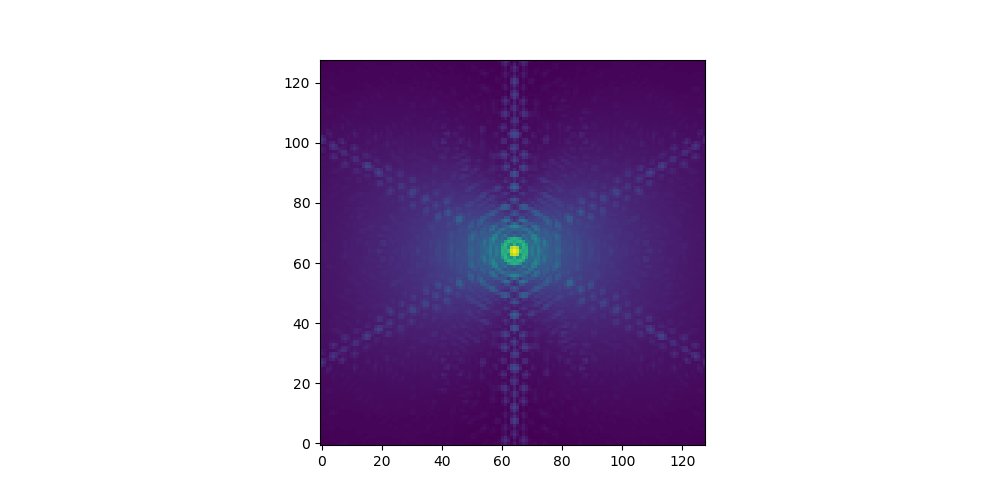
\includegraphics{relay_psf.png}}\phantomsection\label{fig-relay-psf}
\end{figure}


\paragraph{Meta-data%
  \label{meta-data}%
}

\begin{quote}
\begin{alltt}
\begin{lstlisting}[frame=single]
            filename : PSF_SCAO_ConstPSF_0_5off.fits
                name : relay_psf
         temperature : 7
        psf_filename : None
        element_name : default_ro
             warning : Default PSF is NOT field varying. See documentation.
              SIMPLE : True
              BITPIX : 8
               NAXIS : 0
              EXTEND : True
              AUTHOR : Kieran Leschinski
            DATE_CRE : 2019-07-30
            DATE_MOD : 2019-07-30
              SOURCE : AnisoCADO
              STATUS : Best guess for a standard observations
               ETYPE : CONSTPSF
                ECAT : -1
               EDATA : 1
             XOFFSET : 0
             YOFFSET : 5
             z_order : [262, 662]
             include : True
       flux_accuracy : 0.001
      sub_pixel_flag : False
       convolve_mode : full
            wave_key : WAVE0
    normalise_kernel : True
 report_plot_include : True
report_table_include : False
\end{lstlisting}
\end{alltt}
\end{quote}


\subsubsection{SurfaceList: \textquotedbl{}relay\_surface\_list\textquotedbl{}%
  \label{surfacelist-relay-surface-list}%
}

\textbf{Included by default}: \texttt{True}

\textbf{File Description}: list of surfaces in the relay optics

\textbf{Class Description}: <no docstring>

\textbf{Changes}:

\begin{itemize}
\item 2018-11-19 (KL) Added meta data

\item 2019-01-28 (KL) Fixed YAML format in meta data

\item 2020-07-18 (KL) Added all 6 mirrors from the CM16 update pdf

\item 2020-07-18 (KL) Pegged temperature to atmosphere
\end{itemize}


\paragraph{Data%
  \label{id1}%
}

\begin{figure}[H]
\noindent\makebox[\linewidth][c]{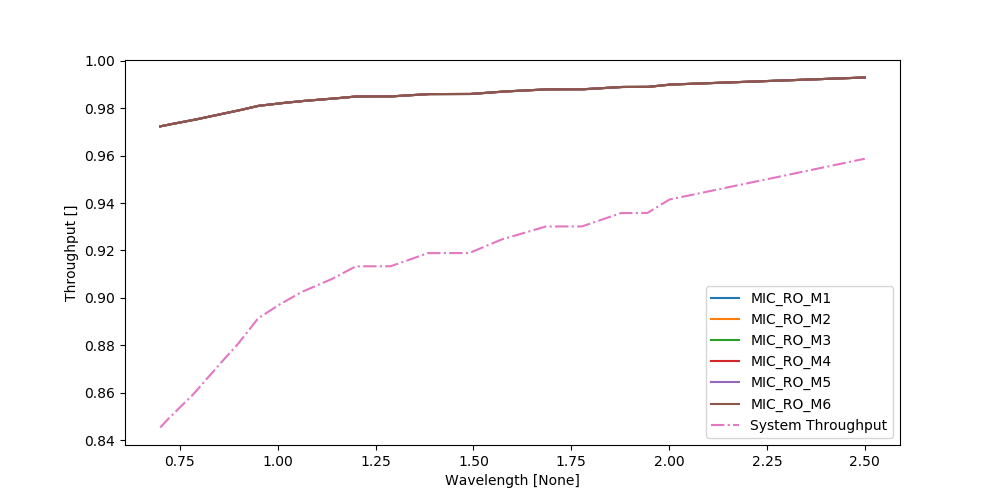
\includegraphics{relay_surface_list.png}}\phantomsection\label{fig-relay-surface-list}
\end{figure}

\setlength{\DUtablewidth}{\linewidth}
\begin{longtable*}[c]{|p{0.111\DUtablewidth}|p{0.068\DUtablewidth}|p{0.068\DUtablewidth}|p{0.068\DUtablewidth}|p{0.195\DUtablewidth}|p{0.121\DUtablewidth}|p{0.333\DUtablewidth}|}
\hline
\textbf{%
name
} & \textbf{%
outer
} & \textbf{%
inner
} & \textbf{%
angle
} & \textbf{%
temperature
} & \textbf{%
action
} & \textbf{%
filename
} \\
\hline
\endfirsthead
\hline
\textbf{%
name
} & \textbf{%
outer
} & \textbf{%
inner
} & \textbf{%
angle
} & \textbf{%
temperature
} & \textbf{%
action
} & \textbf{%
filename
} \\
\hline
\endhead
\multicolumn{7}{c}{\hfill ... continued on next page} \\
\endfoot
\endlastfoot

MIC\_RO\_M1
 & 
0.505
 & 
0.0
 & 
45.0
 & 
!ATMO.temperature
 & 
reflection
 & 
TER\_MICADO\_mirror\_mgf2agal.dat
 \\
\hline

MIC\_RO\_M2
 & 
0.51
 & 
0.0
 & 
10.0
 & 
!ATMO.temperature
 & 
reflection
 & 
TER\_MICADO\_mirror\_mgf2agal.dat
 \\
\hline

MIC\_RO\_M3
 & 
0.184
 & 
0.0
 & 
10.0
 & 
!ATMO.temperature
 & 
reflection
 & 
TER\_MICADO\_mirror\_mgf2agal.dat
 \\
\hline

MIC\_RO\_M4
 & 
0.53
 & 
0.0
 & 
10.0
 & 
!ATMO.temperature
 & 
reflection
 & 
TER\_MICADO\_mirror\_mgf2agal.dat
 \\
\hline

MIC\_RO\_M5
 & 
0.406
 & 
0.0
 & 
20.0
 & 
!ATMO.temperature
 & 
reflection
 & 
TER\_MICADO\_mirror\_mgf2agal.dat
 \\
\hline

MIC\_RO\_M6
 & 
0.406
 & 
0.0
 & 
35.0
 & 
!ATMO.temperature
 & 
reflection
 & 
TER\_MICADO\_mirror\_mgf2agal.dat
 \\
\hline
\end{longtable*}
\label{tbl-relay-surface-list}


\paragraph{Meta-data%
  \label{id2}%
}

\begin{quote}
\begin{alltt}
\begin{lstlisting}[frame=single]
            filename : LIST_RO_SCAO_mirrors.dat
                name : relay_surface_list
         temperature : !ATMO.temperature
        psf_filename : None
        element_name : default_ro
              author : Oliver Czoske, Kieran Leschinski
              source : P12_RelayOptics_Status_2020-06-23-MICADO-CM16-RO-v2.pdf
        date_created : 2018-11-19
       date_modified : 2020-08-17
              status : Design, pre FDR list of stand-alone SCAO relay optics mirrors
                type : mirror:list
          outer_unit : m
          inner_unit : m
          angle_unit : degree
    temperature_unit : deg_C
             z_order : [20, 120, 520]
             include : True
        ignore_wings : False
            wave_min : !SIM.spectral.wave_min
            wave_max : !SIM.spectral.wave_max
           wave_unit : !SIM.spectral.wave_unit
            wave_bin : !SIM.spectral.spectral_resolution
 report_plot_include : True
report_table_include : True
  minimum_throughput : !SIM.spectral.minimum_throughput
             etendue : !TEL.etendue
\end{lstlisting}
\end{alltt}
\end{quote}

\end{samepage}

\end{document}
